\chapter{\uppercase{Design Dataset and Experiments}}\label{Ch:Model_Training}

In this chapter, we will discuss the Dataset Design, Training and Experiments done in this project. The Dataset Design steps started from acquisition and encoding including the essential pre-processing steps, and the justification for their need. Pre-processing steps are data extraction, data cleansing, data format, data encoding techniques used. Also, it contains comparisons between the three techniques used. The training phase started by exploring what the ratio of Training, Testing, and Validation is. Choosing the correct percentage of training dataset compared to the Testing and Validation in Deep learning differs from normal machine learning structure, and it affects the model performance. The results and Discussion phase It explains the results of all the 192 experiments on our dataset. Also, How we assess our model design.

\clearpage

\section{Dataset Design}

In this section, we introduce the dataset acquisition and encoding, including the essential pre-processing steps, and the justification for their need. Pre-processing steps are data extraction, data cleansing, data format, and the data encoding techniques used. This section also contains comparisons between the three techniques used.

The collection of the dataset was one of the most laborious tasks in this project, involving the search for these criteria:

\begin{itemize}
 
 \item \textbf{Datasets availability:} There are old Arabic references which contain many poems, not all of which were available in PDF or Web pages format, and could be difficult to locate.
 
 \item \textbf{The Poem with diacritics:} Some resources have Arabic Poems, but it is difficult to find versions with diacritics.
 
 \item \textbf{The amount of the dataset:} To have a successful project with good results we need a massive amount of data. From the previous work, We did not find this amount of data. The maximum number found was 1.5k. However, We were searching for around 1.5M record of classified poetry.

 
 \item \textbf{Cleansing of this data:} The amount of the datasets which could be considered was limited; alternatively data could be scrapped due to the limited APIs or already-existing datasets in this context.
 
\end{itemize}
To meet the above criteria and overcome it, we applied following:

\begin{itemize}

 \item \textbf{Datasets availability:} We have scrapped the Arabic datasets from two large poetry websites: \textarabic{الديوان}~\cite{diwan}, \textarabic{الموسوعة الشعرية}~\cite{PoetryEncyclopedia2016}. Both were merged into one large dataset, which was open sourced online~\cite{ArabicpoetryDS}.

 \item \textbf{Poems with diacritics:} We tried to get the most verses with the available diacritics, but these are inconsistent; a verse may contain full diacritics, partial diacritics or no diacritics.

 \item \textbf{The size of the dataset:} The total number of verses is 1,862,046 poetic verses; each verse is labeled by its meter (class), the poet who wrote it, and the age which it was written. There are 22 meters, 3701 poets and 11 ages;these are Pre Islamic, Islamic, Umayyad, Mamluk, Abbasid, Ayyubid, Ottoman, Andalusian, the era between Umayyad and Abbasid, Fatimid, and modern. We are only interested in the 16 classic meters attributed to Al-Farahidi, which constitute the majority of the dataset with a total number of 1,722,321 verses. Figure~\ref{Fig:Data_Size_Distribution} shows the distribution of the verses per meter. %@@@ add datasets figures percentage per class
 
 \item \textbf{Cleansing of this data:} Dataset was not sufficiently cleansed for usage in this research, but we have applied cleansing rules explained in detail in the Data Preparation and Cleansing section~\ref{sec:Data_Clens}. We also open sourced all the code scripts used in our online repository~\cite{HCILAB_ArabicPoetry_2018}.
\end{itemize}

\begin{figure}[!t]
 \centering
 \begin{tikzpicture}
 \begin{axis}[
    symbolic x coords={Taweel,
   Kamel,
   Baseet,
   Khafeef,
   Wafeer,
   Rigz,
   Raml,
   Motakarib,
   Sar'e,
   Monsareh,
   Mogtath,
   Madeed,
   Hazg,
   Motadarik,
   Moktadib,
   Modar'e
    },
    xtick=data,
    % the following x label positioning does work here.
    every axis y label/.style= {at={( 0.15, 1.07)}, anchor=north},
    ylabel style={font=\footnotesize},
    xticklabel style = {font=\footnotesize},
    ylabel={Verses},
    height=8cm,
    x=0.4cm,
    x tick label style={rotate=90, anchor=east},
    enlarge y limits=0.07,
    name=left plot,%
    title=(a) \textit{Arabic Dataset},%
    title style={at={(0.5,-.4)}}%
  ]
    \addplot[ybar,color=black,mark=*, only marks,
	    point meta=explicit symbolic] coordinates {
        (Taweel, 416428)
        (Kamel,  370116)
        (Baseet, 244583)
        (Khafeef,     157880)
        (Wafeer,     143148)
        (Rigz,     119286)
        (Raml,     79560)
        (Motakarib,     63613)
        (Sar'e,     59370)
        (Monsareh,     28768)
        (Mogtath,     18062)
        (Madeed,     7808)
        (Hazg,     7468)
        (Motadarik,     5144)
        (Moktadib,     799 )
        (Modar'e,     288 )
    };

    \draw[loosely dotted] (axis cs:Taweel, 0) -- (axis cs:Taweel, 416428);
    \draw[loosely dotted] (axis cs:Kamel,  0) -- (axis cs:Kamel,  370116);
    \draw[loosely dotted] (axis cs:Baseet, 0) -- (axis cs:Baseet, 244583);
    \draw[loosely dotted] (axis cs:Khafeef,0) -- (axis cs:Khafeef,157880);
    \draw[loosely dotted] (axis cs:Wafeer, 0) -- (axis cs:Wafeer, 143148);
    \draw[loosely dotted] (axis cs:Rigz,   0) -- (axis cs:Rigz,   119286);
    \draw[loosely dotted] (axis cs:Raml,   0) -- (axis cs:Raml,   79560);
    \draw[loosely dotted] (axis cs:Motakarib, 0) -- (axis cs:Motakarib, 63613);
    \draw[loosely dotted] (axis cs:Sar'e, 0)   -- (axis cs:Sar'e, 59370);
    \draw[loosely dotted] (axis cs:Monsareh, 0) -- (axis cs:Monsareh,28768);
    \draw[loosely dotted] (axis cs:Mogtath, 0) -- (axis cs:Mogtath, 18062);
    \draw[loosely dotted] (axis cs:Madeed,  0) -- (axis cs:Madeed,  7808);
    \draw[loosely dotted] (axis cs:Hazg,    0) -- (axis cs:Hazg,    7468);
    \draw[loosely dotted] (axis cs:Motadarik,0) -- (axis cs:Motadarik, 5144);
    \draw[loosely dotted] (axis cs:Moktadib, 0) -- (axis cs:Moktadib,  799 );
    \draw[loosely dotted] (axis cs:Modar'e,  0) -- (axis cs:Modar'e,   288 );

\end{axis}



 \end{tikzpicture}%
 \caption{Arabic dataset Meter per class percentage ordered descendingly on x axis vs. corresponding meter name on y axis all class in the left of the red line (less than 1\% assume to be trimmed in some experiments).	}\label{Fig:Data_Size_Distribution}
\end{figure}

\subsection{Data Scraping}\label{sec:Data_Scrap}
To scrape the data from the website: \textarabic{الديوان}~\cite{diwan},is to minimize the problem. Specifically, it should first be ascertained if any "keywords" are set, if used. Then the entire preamble and the complete bibliography are printed. If the same error recurs, the problem might be in the preamble. If so, the preamble is reduced, until the bibliography is printed. Parts are slowly added back to the preamble, until the error occurs again. This may reveal the cause of the warning. We used custom Python scripts for each website, to acquire the verses’ details. The script created with simple usage to pass the link we need to scrape, illustrated below with examples from both websites.

\begin{enumerate}
 \item First example; if we need to scrape a meter from \textarabic{الديوان} the website, for example Al-Tawil \url{https://www.aldiwan.net/poem.html?Word=\%C7\%E1\%D8\%E6\%ED\%E1\&Find=meaning}, we will passed this link to the script and the output file name. The script started scraping and the output was saved in a CSV format. We can obtain an output similar to that in the output in table~\ref{Tab:Aldiwan_Sample}

 \item Second Example; if we need to scrape the same meter from \textarabic{الموسوعة الشعرية} the website (for example Al-Raml \url{https://poetry.dctabudhabi.ae/\#/diwan/poem/126971}), we passed this link to the script and the output file name. The script started scraping and the output was saved in a CSV format. We can obtain an output similar than the output in table~\ref{Tab:ElMosoaa_Sample}

We scraped all the available datasets on both websites and merged them based on the common columns. Then we started the Data preparation tasks. It should be mentioned that not all diacritics were correctly available on all the websites. Nor did we work to generate the diacritics for those datasets. We therefore depended on available data, which remained unchanged. The following sections relate to correction, preparation, and cleansing of the current datasets.

 \subsection{Data Preparation and Cleansing}\label{sec:Data_Clens}

Data preparation and cleansing tasks were divided into multi-stages:

 \begin{itemize}
 \item All scraped datasets were merged into one CSV file with a selection of the common columns in each file.
 \item The duplicates rows were removed from the files in case of any joined rows between both websites.
 \item The datasets on the 16 meters required were filtered, as some data belonged to other non-famous or not original meters.
 \item Many unnecessary or useless white spaces were removed.
 \item Removal of non-Arabic characters and other web symbols.
 \item Diacritical mistakes were rectified, such as the removal of one of two consecutive harakats. 
 \item Removal of any \textit{harakah} occurring after a white space. 
 \item Shadaa~\ref{def:shadaa_definition} was factored to its original format, explained in this example~\ref{Tab:Diacritics_Dal} previously.
 \item Tanween~\ref{def:tanween_definition} was also factored to its original format, explained in this example~\ref{Tab:Tanween_Dal} previously.\footnote{\textit{We ignored the factorization of Alef-Mad \textarabic{(آ)} in our data preparation and transformation, thus saving more memory and shortening our encoding vectors.}}
 \end{itemize}

 We need to highlight that the last two points are not a handcrafted feature. They involve a factorization of the letter to its original format. This factorization will affect the size of the data in the memory, and the letter representation in the vector. We will explain this part in detail in the next chapter on the encoding mechanism and the impact of the encoding type in the model training time and performance.

 % \clearpage
 % table: dal with diacritics
 \begin{table}[!t]
 \centering
 \begin{tabular*}{\textwidth}{c @{\extracolsep{\fill}}c c c c c}
  % \hline
  \toprule
  \textbf{\small{\textarabic{البيت}}} & \small{\textbf{\textarabic{الشطر الأيسر}}} & \small{\textbf{\textarabic{الشطر الأيمن}}} &
                                  \small{\textbf{\textarabic{البحر}}} & \small{\textbf{\textarabic{الشاعر}}} \\
                                  % \hline
  \midrule
  \makecell{\textarabic{رَجا شافع نسج المودّة بيننا}\\ \textarabic{ولا خيرَ في ودّ يكون بشافع}} &
                         \textarabic{ولا خيرَ في ودّ يكون بشافع} &              \textarabic{رَجا شافع نسج المودّة بيننا} &              \textarabic{الطويل}&
                                                                             \textarabic{ابن نباته المصري}\\
  
                                                                             % \hline
  \bottomrule
 \end{tabular*}
 \caption{Aldiwan scraping output example }\label{Tab:Aldiwan_Sample}
 \end{table}


 % table: dal with diacritics
 \begin{table}[!t]
 \centering
 \begin{tabular*}{\textwidth}{c @{\extracolsep{\fill}}c c c c c c c c c}
  % \hline
  \toprule
  \small{\textbf{\#}} &
       \small{\textbf{\textarabic{البيت}}} &
                 \small{\textbf{\textarabic{الشطر الأيمن}}}&      \small{\textbf{\textarabic{الشطر الأيسر}}} &
                                             \small{\textbf{\textarabic{البحر}}}&         \small{\textbf{\textarabic{القافية}}}& \small{\textbf{\textarabic{الديوان}}}&        \small{\textbf{\textarabic{الشاعر}}}&
                                                                                                   \small{\textbf{\textarabic{العصر}}}\\
                                                                                                   % \hline
  \midrule
  1 &   
   \makecell{\textarabic{من يرد مورد حب} \\ \textarabic{ظمأ بالشوق يزدد}} &
                     \textarabic{ظمأ بالشوق يزدد} &              \textarabic{من يرد مورد حب} &              \textarabic{الرمل}&
                                                                     \textarabic{د}&
                                                                         \makecell{\textarabic{الديوان} \\ \textarabic{الرئيسي}}&
                                                                                       \makecell{\textarabic{يعقوب الحاج}\\ \textarabic{ جعفر التبريزي}}&
                                                                                                        \textarabic{الحديث}\\
  
                                                                                                        % \hline
  \bottomrule
 \end{tabular*}
 \caption{Al-Mosoaa Elshearyaa scraping output example }\label{Tab:ElMosoaa_Sample}
 \end{table}
\end{enumerate}


\subsection{Data Encoding}\label{Ch:Data_Encoding}

As explained, we collected the dataset and checked the data from any quality issues. The next step was to prepare the data representation for model training. This change in the data structure is named Data Encoding.

\subsubsection{Encoding in English}

\begin{itemize}
 \item \textbf{Work embedding Encoding in English:} The concept of data encoding was first introduced by Bengio et al. (2003)~\cite{Bengio2003}. They used an embedding lookup table as a reference and mapped every word to this lookup. They used the resulting dense vectors as input for language modeling. There are many works to improve the word embedding one of them. Collobert et al. (2011)~\cite{Collobert_2011} proposed improvement of word embedding task and proved the versatility of word embedding in many NLP tasks. Other works proposed by Mikolov et al. (2013)~\cite{Mikolov_2013}; and Pennington et al. (2014)~\cite{Pennington_2014} ] show the maturity of word embedding, which is currently the most used encoding technique in the neural network based natural language processing.

 \item \textbf{Character Level Encoding in English} : All the previous work focused on word embedding encoding, but in thisresearch problem, we work not on word level; instead we focus on character level encoding as an input feature of the model. There is much research based on character level encoding. Kim et al. (2015)~\cite{Kim_2015} used character level embedding to construct word level representations to work on vocabulary problems. Chiu and Nichols (2015)~\cite{Chiu_2015} also used character embeddings with a convolutional neural network for named entity recognition. Lee et al. 2017]~\cite{ijcai_2017} used character embeddings for personal name classification, using Recurrent Neural Networks.

\end{itemize}

\subsubsection{Character Level Encoding in Arabic}\label{sec:Char_Level_Arabic}

Working on Arabic language embedding based on the character level has attracted little attention from the research community. Potdar et al. (2017) ~\cite{Potdar_2017} have undertaken a comparative study on six encoding techniques. Of interest is the comparison of \textit{one-hot} and \textit{binary}. They have used Artificial Neural Network for evaluating cars, based on seven ordered qualitative features. The accuracy of the model was the same in both encoding \textit{one-hot} and \textit{binary}. Agirrezabal et al. (2017) ~\cite{Agirrezabal_2017} show that representations of data learned from character-based neural models are more informative than the ones from hand-crafted features.

This research makes a comparative study between different encoding techniques \textit{binary} and \textit{one-hot}. We also provide some new encoding method specific to Arabic letters, and we will see the effect of this on our problem. We will show the efficiency of every technique based on performing model training and model running time performance.

Generally, a character will be represented as an $n$ vector. Consequently, a verse would be an $n \times p$ matrix, where $n$ is the character representation length and $p$ is the verse’s length. Where $n$ varies from one encoding to another, we have used \textit{one-hot} and \textit{binary} encoding techniques and proposed a new encoding, the \textbf{\textit{two-hot}} encoding.

Arabic letters have a feature related to the diacritics; To explain this feature we will take an example based on \textit{\textit{one-hot}} encoding. This feature is related to how we will treat the character with a diacritic. Arabic letters are 36 + white space as a letter. So, the total is 37. Any letter represented as a vector $37 \times 1$. Let's take an example a work such as \textarabic{مرحبا} having 5 letters encoded as a $37 \times 5$ matrix. If it came with diacritics such as \textarabic{مَرْحَبَا} and we need to represent the letters as \textit{one-hot} encoding we will consider every letter and diacritics as a separate letter. So, it will be 5 character and 4 diacritics. The vector shape will be $41 \times 9$.

One diacritical feature of Arabic letters can be explained by an example based on \textit{one-hot} encoding. 
This feature is related to our treatment of characters with diacritics. 
There are 36 Arabic letters. Including the white space, the total is 37. 
Any letter represented as a vector $37 \times 1$. For example, a work such as \textarabic{مرحبا} has 5 letters encoded as a $37 \times 5$ matrix. 
If it came with diacritics such as \textarabic{مَرْحَبَا} and we needed to represent the letters using \textit{one-hot} encoding, we would consider every letter and diacritic as a separate letter, thus 5 characters and 4 diacritics. The vector shape will be $41 \times 9$.

One of the main reasons for focusing on the encoding is the \textit{RNN} training. 
Different numbers of time steps in \textit{RNN} cells, and different input vector dimensions based on the input will lead to a standard architecture for the model and permit both work with and without diacritics to show the effect of the model learning on the same architecture.

To achieve the model architecture unification, we proposed three different encoding systems: \textit{one-hot}, \textit{binary}, and the novel encoding system developed in this project \textit{two-hot}. All three are explained in the next three subsections.

\begin{figure*}[!t]
 \centering
 \begin{tikzpicture}
    \node at (-12,0){\begin{tikzpicture}   
  % Rectangles
  % the space between each rectangular
  \def \x {0.57} 
  \def \s {1} % I'll use it to shift to right
  % A list of letters <3
  \newcommand\letters{{"ا","بَ","حَ", "رْ", "مَ"}}

  % Rectangle
  \def \length {2.95}
  \foreach \j in {0,...,4} 
  \draw [rounded corners=1pt] (\s+\x*\j, 0) rectangle (\s+0.5+\x*\j, \length) 
  node[above, xshift=-0.25cm]
  {\textarabic{\pgfmathparse{\letters[\j]}\pgfmathresult}};

  % Above Annotation
  % Cell line
  % 0.25*10+0.09 = 2.59
  \def \d {3.9 - 0.15}
  \draw (\s+0.25-0.007, 3.9 ) -- (\s+2.53+0.007, 3.9 ); % the main bar
  \draw (\s+0.25, 3.9 ) -- (\s+0.25, \d ); % sub bar #ا
  \draw (\s+0.25*3+0.03, 3.9 ) -- (\s+0.25*3+0.03, \d ); % sub bar #ب
  \draw (\s+0.25*5+0.15, 3.9+0.15 ) -- (\s+0.25*5+0.15, \d ) 
  node[above, yshift=0.3cm]{\textarabic{مَرْحَبَا}}; % sub bar #ح
  \draw (\s+0.25*7+0.2, 3.9 ) -- (\s+0.25*7+0.2, \d ); % sub bar #ر
  \draw (\s+2.53, 3.9 )  -- (\s+2.53, \d );  % sub-bar #م

  % adding numbers, vector ا
  \node at (\s+0.25, \length - 0.25)    {1}; % the top number; using -
  \node at (\s+0.25, \length - 0.6)     {0};
  \node at (\s+0.25, \length - 0.95)    {0};
  \node at (\s+0.25, \length - 1.3)     {0};
  \node at (\s+0.25,  1.1)     {\vdots};
  % \node at (\s+0.25, \length - 1.65)    {0};
  % \node at (\s+0.25, \length - 2)       {0};
  % \node at (\s+0.25, \length - 2.35)    {0};
  \node at (\s+0.25, \length - 2.7)     {0};

  % distance between vectors elements
  \def \d {0.07}
  % adding numbers, vector ب
  \node at (\s+0.25*3+\d, \length - 0.25)    {0}; % the top number; using -
  \node at (\s+0.25*3+\d, \length - 0.6)     {\vdots};
  % \node at (\s+0.25*3+\d, \length - 0.95)    {0};
  \node at (\s+0.25*3+\d, \length - 1.18)     {1};
  \node at (\s+0.25*3+\d, 1.28) {\vdots};
  \node at (\s+0.25*3+\d, \length - 2.35)    {0};
  \node at (\s+0.25*3+\d, 0.25) {0}; % The bottom  number


  % adding numbers, vector ح
  \node at (\s+0.25*5+\d*2, \length - 0.25)    {0}; % the top number; using -
  \node at (\s+0.25*5+\d*2, \length - 0.6)     {\vdots};
  \node at (\s+0.25*5+\d*2, \length - 1.35)     {1};
  \node at (\s+0.25*5+\d*2, 1.18) {\vdots};
  \node at (\s+0.25*5+\d*2, \length - 2.35)    {0};
  \node at (\s+0.25*5+\d*2, 0.25) {0}; % The bottom  number

  % adding numbers, vector ر
  \node at (\s+0.25*7+\d*3, \length - 0.25)    {0}; % the top number; using -
  \node at (\s+0.25*7+\d*3, \length - 0.6)     {0};
  \node at (\s+0.25*7+\d*3, \length - 0.95)     {0};
  \node at (\s+0.25*7+\d*3, \length - 1.33)     {\vdots};
  \node at (\s+0.25*7+\d*3, 1.07) {1};
  \node at (\s+0.25*7+\d*3, \length - 2.2)    {\vdots};
  \node at (\s+0.25*7+\d*3, 0.25) {0}; % The bottom  number

  % adding numbers, vector م
  \node at (\s+0.25*9+\d*4, 3 - 0.25) {0}; % the top number; using -
  \node at (\s+0.25*9+\d*4, 3 - 0.69) {0};
  \node at (\s+0.25*9+\d*4, 0.25) {0};
  \node at (\s+0.25*9+\d*4, 0.25*4 - 0.1) {\vdots};
  \node at (\s+0.25*9+\d*4, 0.9 + 0.4) {1};
  \node at (\s+0.25*9+\d*4, 1.3 + 0.6) {\vdots};

  % Vector size annotations.
  % figures starts at x = 1
  \def \d {0.6} % Annotation x=0.4
  \draw[arrows=->] (\d, 1.7) -- (\d, 2.9); % up-line
  \draw[arrows=<-] (\d, 0.1) -- (\d, 1.1) node[above, yshift=0.07cm]
  {\small{181}};
  % bottom-line

  % \draw[arrows=<-] (\s+0.1, -0.4) -- (\s+1.19, -0.4) node[right, xshift=0.05cm] {\small{5}};
  % \draw[arrows=->] (\s+1.2+0.5, -0.4) -- ( \s+2.7,-0.4);
\end{tikzpicture}%

%%% Local Variables:
%%% mode: latex
%%% TeX-master: "../main"
%%% End:

};
    \node at (-7,0){\begin{tikzpicture}[x=1cm,y=1cm]

  % Rectangles
  % the space between each rectangular
  \def \x {0.57} 
  \def \s {1} % I'll use it to shift to right
  % A list of letters <3
  \newcommand\letters{{"ا","بَ","حَ", "رْ", "مَ"}}

  % \draw[step=0.2, gray, very thin, red] (1,-0.5) grid (4,4);

  % Rectangulars
  \def \length {2.95}
  \foreach \j in {0,...,4} 
  \draw[rounded corners=1pt] (\s+\x*\j, 0) rectangle (\s+0.5+\x*\j, \length) 
  node[above, xshift=-0.25cm]
  {\textarabic{\pgfmathparse{\letters[\j]}\pgfmathresult}};

  % Above Annotatios
  % Cell line
  % 0.25*10+0.09 = 2.59
  \def \d {3.9 - 0.15}
  \def \z {0.2}
  \draw (\s+0.25-0.007, 3.9 ) -- (\s+2.53+0.007, 3.9 ); % the main bar
  \draw (\s+0.25, 3.9 ) -- (\s+0.25, \d ); % sub bar #ا
  \draw (\s+0.25*3+0.03, 3.9 ) -- (\s+0.25*3+0.03, \d ); % sub bar #ب
  \draw (\s+0.25*5+0.15, 3.9+0.15 ) -- (\s+0.25*5+0.15, \d ) 
  node[above, yshift=0.3cm]{\textarabic{مَرْحَبَا}}; % sub bar #ح
  \draw (\s+0.25*7+0.2, 3.9 ) -- (\s+0.25*7+0.2, \d ); % sub bar #ر
  \draw (\s+2.53, 3.9 )  -- (\s+2.53, \d );  % sub-bar #م

  % adding numbers, vector ا
  \node at (\s+0.25, \length - 0.25)    {0}; % the top number; using -
  \node at (\s+0.25, \length - 0.6)     {0};
  \node at (\s+0.25, \length - 0.95)    {0};
  \node at (\s+0.25, \length - 1.3)     {0};
  \node at (\s+0.25, \length - 1.65)    {0};
  \node at (\s+0.25, \length - 2)       {0};
  \node at (\s+0.25, \length - 2.35)    {0};
  \node at (\s+0.25, \length - 2.7)     {1};

  % distance between vectors elements
  \def \d {0.07}
  % adding numbers, vector ب
  \node at (\s+0.25*3+\d*1, \length - 0.25)    {0}; % the top number; using -
  \node at (\s+0.25*3+\d*1, \length - 0.6)     {0};
  \node at (\s+0.25*3+\d*1, \length - 0.95)    {1};
  \node at (\s+0.25*3+\d*1, \length - 1.3)     {0};
  \node at (\s+0.25*3+\d*1, \length - 1.65)    {0};
  \node at (\s+0.25*3+\d*1, \length - 2)       {1};
  \node at (\s+0.25*3+\d*1, \length - 2.35)    {1};
  \node at (\s+0.25*3+\d*1, \length - 2.7)     {1};


  % adding numbers, vector ح
  \node at (\s+0.25*5+\d*2, \length - 0.25)    {0}; % the top number; using -
  \node at (\s+0.25*5+\d*2, \length - 0.6)     {0};
  \node at (\s+0.25*5+\d*2, \length - 0.95)    {1};
  \node at (\s+0.25*5+\d*2, \length - 1.3)     {0};
  \node at (\s+0.25*5+\d*2, \length - 1.65)    {1};
  \node at (\s+0.25*5+\d*2, \length - 2)       {0};
  \node at (\s+0.25*5+\d*2, \length - 2.35)    {1};
  \node at (\s+0.25*5+\d*2, \length - 2.7)     {1};

  % adding numbers, vector ر
  \node at (\s+0.25*7+\d*3, \length - 0.25)    {1}; % the top number; using -
  \node at (\s+0.25*7+\d*3, \length - 0.6)     {0};
  \node at (\s+0.25*7+\d*3, \length - 0.95)    {0};
  \node at (\s+0.25*7+\d*3, \length - 1.3)     {1};
  \node at (\s+0.25*7+\d*3, \length - 1.65)    {1};
  \node at (\s+0.25*7+\d*3, \length - 2)       {0};
  \node at (\s+0.25*7+\d*3, \length - 2.35)    {1};
  \node at (\s+0.25*7+\d*3, \length - 2.7)     {1};

  % adding numbers, vector م
  \node at (\s+0.25*9+\d*4, \length - 0.25)    {0}; % the top number; using -
  \node at (\s+0.25*9+\d*4, \length - 0.6)     {0};
  \node at (\s+0.25*9+\d*4, \length - 0.95)    {1};
  \node at (\s+0.25*9+\d*4, \length - 1.3)     {1};
  \node at (\s+0.25*9+\d*4, \length - 1.65)    {1};
  \node at (\s+0.25*9+\d*4, \length - 2)       {1};
  \node at (\s+0.25*9+\d*4, \length - 2.35)    {0};
  \node at (\s+0.25*9+\d*4, \length - 2.7)     {1};

  % Vector size annotations.
  % figures starts at x = 1
  \def \vColumn {0.6} % Annotation x=0.4
  \draw[arrows=->] (\vColumn, 1.7) -- (\vColumn, 2.9); % up-line
  \draw[arrows=<-] (\vColumn, 0.1) -- (\vColumn, 1.1) node[above, yshift=0.07cm] {\small{8}};
  % bottom-line

  % \draw[arrows=<-] (\s+0.1, -0.4) -- (\s+1.19, -0.4) node[right, xshift=0.05cm] {\small{5}};
  % \draw[arrows=->] (\s+1.2+0.5, -0.4) -- ( \s+2.7,-0.4);

\end{tikzpicture}


%%% Local Variables:
%%% mode: latex
%%% TeX-master: "../main"
%%% End:

};
    \node at (0,0){% Defining a new box
\newsavebox{\columnVector}
% Populating the box
\savebox{\columnVector}{$\left[\begin{smallmatrix}k\\m\end{smallmatrix}\right]$}

\begin{tikzpicture}

  % The grid
  % \draw[step=0.5, gray!40, very thin] (0,0) grid (6,4);

  \def \recWidthA {0.5}
  \def \yStartA   {1.5}
  \def \yEndA     {3}
  \def \xStartA   {1.5}
  \def \xEndA     {0.5}
  \def \xStartB   {0}
  \def \yStartB   {1}
  \def \xEndB     {2}
  \def \yEndB     {3.5}
  \def \half      {\yEndA/2 - \yStartA/2}
  \def \xStartC   {3 +0.5}
  \def \yStartC   {0.5 -.1}
  \def \xEndC     {3.5 +0.5}
  \def \yEndC     {4 +.1 }
  \def \shiftMargin {0.3}
  \newcommand\numbers{{0.25, 0.6, 0.95, 1.3, 1.65, 2, 2.35, 2.7}}

  % Rectangle A
  \draw[rounded corners=2pt] (\xStartA, \yStartA) rectangle (\xStartA + \recWidthA, \yEndA)
  node [above, xshift=-.25cm] {\textarabic{◌َ}};
  % Populating the rectangle A
  \node at (0.25 + \xStartA, 3 -\numbers[0]) {1};
  \foreach \j in {1,...,3}
  \node at (0.25 + \xStartA, \yEndA -\numbers[\j]) {0};

  % Annotation A
  \node at (\xStartA-\shiftMargin, \yStartA + \half) {\small 4};
  \draw[arrows=-angle 90, very thin] (\xStartA-\shiftMargin, \yStartA + \half +.3) -- (\xStartA-\shiftMargin, \yEndA -0.1);
  \draw[arrows=angle 90-, very thin] (\xStartA-\shiftMargin, \yStartA + .1) -- (\xStartA-\shiftMargin, \yStartA + \half -.3);

  % Rectangle B
  \draw[rounded corners=2pt] (\xStartB +0.5, \yStartB) rectangle (\yStartB +0.5 -1.5, \yEndB)
  node[above, xshift=0.25cm] {\textarabic{ب}};
  \node at (\xStartB +0.25, \yEndB -\numbers[0]) {0};
  \node at (\xStartB +0.25, \yEndB -\numbers[1]) {1};
  \node at (\xStartB +0.25, \yEndB -\numbers[2]) {0};
  \node at (\xStartB +0.25, \yEndB -\numbers[3]) {0};
  \node at (\xStartB +0.25, \yEndB -\numbers[4] ) {\vdots};
  \node at (\xStartB +0.25, \yStartB +\numbers[0]) {0};

  % Annotation B
  \node at (-\shiftMargin, \yStartA + \half) {\small 37};
  \draw[arrows=-angle 90, very thin] (-\shiftMargin, \yStartA + \half +.3) -- (-\shiftMargin, \yEndB -0.1);
  \draw[arrows=angle 90-, very thin] (-\shiftMargin, \yStartB + .1) -- (-\shiftMargin, \yStartA + \half -.3);

  \node at (0.8, \yStartA +\half) {$+$};
  \node at (2.5 + .02, \yStartA +\half) {$=$};

  % Rectangle C
  \draw[rounded corners=2pt]  (\xStartC, \yStartC) rectangle (\xEndC, \yEndC)
  node[above, xshift=-0.25cm] {\textarabic{بَ}};
  ;
  \node at (\xStartC +0.25, \yEndC -\numbers[0]) {1};
  \node at (\xStartC +0.25, \yEndC -\numbers[1]) {0};
  \node at (\xStartC +0.25, \yEndC -\numbers[2]) {0};
  \node at (\xStartC +0.25, \yEndC -\numbers[3]) {0};

  \node at (\xStartC +0.25, \yEndC -\numbers[4] -.2) {0};
  \node at (\xStartC +0.25, \yEndC -\numbers[5] -.2) {1};
  \node at (\xStartC +0.25, \yEndC -\numbers[6] -.2) {0};
  \node at (\xStartC +0.25, \yEndC -\numbers[7] -.2) {\vdots};
  \node at (\xStartC +0.25, \yStartC +\numbers[0]) {0};

  % Annotation
  \node at (\xStartC -\shiftMargin, \yStartA +\half) {\small 41};
  \draw[arrows=-angle 90, very thin]  (\xStartC -\shiftMargin, 2.5) -- (\xStartC -\shiftMargin, \yEndC -0.1);
  \draw[arrows=angle 90-, very thin]  (\xStartC -\shiftMargin, 0.5) -- (\xStartC -\shiftMargin, 2);

  \draw [decorate,decoration={brace,amplitude=2pt,mirror,raise=2pt}, very thin]
  (\xEndC +\shiftMargin -.1, 2.5 +.2) -- (\xEndC +\shiftMargin  -.1, \yEndC -0.1);
%  node [right, midway, xshift=0.2cm, yshift=0.1cm] {\tiny $4 \times 1$ diacritic vector};

  \draw [decorate,decoration={brace,amplitude=2pt,mirror,raise=2pt}, very thin]
  (\xEndC +\shiftMargin -.1, 0.5) -- (\xEndC +\shiftMargin -.1, 2.4);
%  node [right, midway, xshift=0.2cm, yshift=0.1cm] {\tiny $37 \times 1$ letter vector};


  \node [rectangle, text width= 5em,font=\footnotesize] at (5.6, 3.4)
    {\scriptsize $4 \times 1$ letter vector which represents \textarabic{◌َ}};

  \node [rectangle, text width= 5em,font=\footnotesize] at (5.6, 1.4)
    {\scriptsize $37 \times 1$ letter vector which represents \textarabic{ب}};

  % \node at (0.25, 0.5) {$\bm m$};
  % \node at (1.5 +.25, 0.5 +0.5) {$\bm k$};
\end{tikzpicture}

%%% Local Variables:
%%% mode: latex
%%% TeX-master: "../main"
%%% End:

};
    \node at (-12+0.3,-3){(a) \textit{One-Hot}};
    \node at (-7+0.3, -3){(b) \textit{Binary}};
    \node at (0-0.5,  -3){(c) \textit{Two-Hot}};
\end{tikzpicture}


 \caption{Different encoding mechanisms%: \One-hot, \textit{binary}, and \textit{two-hot} encoding. Using the word example %\textarabic{مَرْحَبَا} \textit{one-hot} encoding is applied using $n$-letter alphabet $n = 181$ in Arabic. Same word encoded using \textit{binary} encoding where the vector length $n = \ceil*{\log_2 l}$, $l \in \{181\}$. \textit{two-hot} encoding is applied by stacking $\bm k_{4 \times 1}$ on the top of $\bm m_{37 \times 1}$, giving the $Two-hot_{41 \times 1}$ \usebox{\columnVector}, which represents a letter and its diacritic simultaneously. 
 }~\label{Fig:One_binary_Encoding}
\end{figure*}



\begin{description}

 \item[\textbf{\textit{One-hot} encoding}] In this encoding system, we assume the letter with the diacritic as one unit. So, for example, \textarabic{د} represented as letter differs than (\textarabic{دَ, دِ, دُ, دْْ}). Now every letter is represented 5 times (one without diacritic and four times with different diacritics), giving combinations $36 \times 5$ besides the white-space character. Hence, the total is $181 \times 1$. Henceforth, we have 181 Arabic alphabetic characters represented in the \textit{one-hot} encoding, which we employ to encode verses. (Figure~\ref{Fig:One_binary_Encoding}).

 It should be noted that that \textit{one-hot} encoding technique is one of the famous techniques in
 encoding problems. We will not compare encoding techniques in these sections. We will, 
 however, discuss it in detail in model results. Moreover, the implementations of the \textit{one-hot} is
 trivial. We need to focus on the size for every letter which is $181 \times 1$;meaning if we have
 a verse with 82 characters, it will result in a matrix $181 \times 82$. This would require very 
 large memory.

 \item[\textbf{\textit{Binary Encoding}}] The idea is to represent a letter with an $n \times 1$ vector which contains a unique combination of ones and zeros. $n =\ceil*{\log_2} l$ where $l$ is the alphabet length, and $n$ is a sufficient number of digits to represent $l$ unique \textit{binary} combinations. For example a phrase like this \textarabic{مَرْحَبا} has 5 characters. figure~\ref{Fig:One_binary_Encoding} shows how it is encoded as a $8 \times 5$ matrix, which saves 22.6 times memory compared to \textit{one-hot}, and reduces the model input dimensions significantly. On the other hand, the input letters share some features due to the \textit{binary} representation as shown in figure~\ref{Fig:One_binary_Encoding}.

 \item[\textbf{\textit{two-hot} encoding}] This is an intermediate technique which takes the advantages of the previous two encoding techniques. In it, we encode the letter and its diacritic separately as two \textit{one-hot} vectors, hence the letter is encoded as $37 \times 1$ \textit{one-hot} vector and the diacritic is encoded as $4 \times 1$ \textit{one-hot} vector, then both vectors are stacked to form one $41 \times 1$ vector (Figure~\ref{Fig:One_binary_Encoding}).

 We thus reduced the vector dimension from 181 to 41, and also minimized the number of shared features between vectors to the maximum one at each vector. 

\end{description}

\subsubsection{Categorical Values Encoding}\label{sec:label_encoder}

Machine Learning uses the encoding techniques to transform the categorical data (class label or text) into numbers. 
This will make it easy for the predictive model to understand our label in an easy representation. 
Some encoding techniques are \textit{label encoding, one hot encoder, and custom \textit{binary} encoding}. 
All these encodings will convert the categorical to numerical values, but in different ways. 
For example, Label encoding can transform the following labels: (apple, orange, banana) to (0,1,2) as a numeric representation. 
As explained in the previous subsection, \textit{one-hot} encoding could transform the labels to ([1,0,0],[0,1,0],[0,0,1]). 
In this research, we used the label encoding for label encoding to the meter’s class, using the \textit{Sklearn} library in Python~\cite{scikit-learn}. The categorical encoding technique has no effect on the results. However, there is some difference in the execution and running time performance.

\clearpage

\section{Model Training}
In a normal machine learning project, the dataset would be divided into approximately 60\% training, 30\% testing and 10\% validation. However, in The Deep Learning, the amount of data profoundly affects the model performance. 
Hence, the more data fed as training, the more performance results the model can achieve on test data (Assuming regularization and the required generalization were conducted in the model training phase). 
The main reason to change the split size is due to the size of the dataset we previously worked on; for example 1\% of 1M sample is 10k, which is big enough for such experiments. 
However, if we work on a 10k sample, we need around 30\% 3k sample to have confidence in our model. It therefore depends on the problem and size of the dataset.

The current research addresses Poem Comprehensive Dataset (PCD)~\cite{ArabicpoetryDS}. We are interested in the 16 classic meters, attributed to Al-Farahidi. These meters comprise the majority of the dataset with a total number of 1,722,321 verses. Figure~\ref{Fig:Data_Size_Distribution} shows an ordered bar chart based on the number of verses per meter. We trained all our models based on 80\%, around 1,377,856 verses. Our testing data (development) is 10\%, around 172,232 verses, and our Validation data around 172,232 verses.

We can show the training phase designed as a data representation configuration and an RNN configuration. The number of experiments is the cross product of both data representations and RNN configuration; for example, If we have 12 data representations and 12 RNN configurations, the total number of experiments will be 144. It should be emphasised that:

\begin{itemize}
 \item Data representation feature is a general feature applied to the dataset, not a hand-drafted feature. More details on~\ref{Sec:Data_Rep_Param}.
 \item Data representation feature is affected by Arabic language pronunciation, and some features provide more information than others.
 \item RNN configurations are the parameters related to the Network model development training, and are used after many experiments to find and tune the best configurations. This means we did more than the number of experiment written in this research but publish only the best results overall. More details are provided in sec~\ref{Sec:Rnn_Param}.
 \item The number of verses (344,464) used in testing and validation is significant, confirming that the model was tested on all types of verses and inspiring confidence in the results.

\end{itemize}

\subsection{Parameters of Data Representation}\label{Sec:Data_Rep_Param}

Arabic language parameters have the following types: Diacritics, Trimming, and Encoding. Every type has its effect on the data and the performance on the model learning rate. Each is explained in detail in the following subsections.

\subsubsection{Diacritics}

The Arabic dataset contains the verse with diacritics. We can feed the network the characters with and without diacritics. With diacritics, it will be much easier for the network to learn, since they provide more information on the pronunciation. Moreover, they provide more information relating to the vowel and consonant sounds in the letters. However, as we discussed in Data Encoding Chapter~\ref{Ch:Data_Encoding}, the inclusion or otherwise of diacritics has the same length in input vector size.


\subsubsection{Trimming Small Classes}

The Arabic poem dataset, as stated in Figure~\ref{Fig:Data_Size_Distribution}, is unbalanced. Hence, as part of our research, we consider the dataset representation as a Full dataset and Trimmed dataset. This allows us to study the effect of this unbalance. We not only explore the impact of the unbalanced dataset, but also apply a technique to solve this issue~\ref{Sec:W_Loss}. The trimmed classes are five classes which have less than 1\% of the total dataset. We present these classes as all the classes on the left side of the horizontal red line in Figure~\ref{Fig:Data_Size_Distribution}. Therefore, the classes after trimming total 11, and in the Full dataset all 16 meters are presented.

\subsubsection{Encoding Techniques}

As explained previously, there are three different encoding methods~\ref{Ch:Data_Encoding}. Although all carry the same information, it was expected that every encoding has its own behaviors (as below):

\begin{itemize}
 \item \textbf{Running Time}: It was expected that the running time would differ from one encoding type to others. This information is important if someone is conducting an experiment with limited time and needs the results as fast as possible.
 \item \textbf{Required Resources}: It was expected that different resources will be required from one encoding type to others. This information is important if someone has an experiment with limited resources.
 
 \item \textbf{Learning Rate}: Some encoding will learn faster than others (Note: Learning Rate not the overall performance) for example, one encoding can achieve 80\% on training performance after four epoch, but another one can reach the same percentage after 20\% epoch.
 \item \textbf{Overall Performance}: The final performance percentage which can be achieved with each encoding technique. (Note: the best learning rate may be the method which takes most time.) Therefore, the researcher who will use this encoding should decide which one will be used based on the criteria needed.

 \item \textbf{Overall Performance}: The final performance percentage which can be achieved with every encoding technique (Note: the best can be the worst in learning rate or the method which take much time). So, the researcher who will use this encoding should decide which one will be used based on the criteria needed.

\end{itemize}

\subsubsection{Data Representation Matrix}

The data representation matrix is the cross product of the Diacritics 2, Data Encoding 3, and Trimming 2: total 12 combinations table~\ref{Tab:Data_Representation_Matrix} shows this matrix combination. Example (With diacritic + \textit{one-hot} + Full)


\begin{table}[t]
 \centering
 \begin{tabular}{c c c c c c}
 \hline
 \textbf{\#} & \textbf{Diacritic} & \multicolumn{3}{c}{\textbf{Encoding Types}} & \textbf{Trimming} \\
 
 \hline
 1 & With diacritic & \textit{one-hot} & \textit{two-hot} & \textit{binary} & Full \\
 \hline
 2 & Without diacritic & \textit{one-hot} & \textit{two-hot} & \textit{binary} & Trimmed \\
 \hline
 \end{tabular}
 \caption{Data Representation Combination Matrix}\label{Tab:Data_Representation_Matrix}
\end{table}


% \begin{figure}[H]
% \centering
% \begin{tikzpicture}
%  
\begin{axis}
[
    axis lines*=left,
    title=Arabic Dataset Classes Percentage \%,
    xbar,
    width=17cm,
    height=14cm,
    xlabel={},
    symbolic y coords={Taweel, Kamel,Baseet,Khafeef,Wafeer,Rigz,Raml,Motakarib,Sar'e,Monsareh,Mogtath,Madeed,Hazg,Motadarik,Moktadib,Modar'e},
    ytick=data,
    xmin=0,
    xmax=.4, 
%    point meta={x*100},
    xtick={0.01,0.05,0.1,0.15,.2,.25,.3,.35},
    xticklabel={\pgfmathparse{\tick*100}\pgfmathprintnumber{\pgfmathresult}\%},
    point meta={x*100},
    nodes near coords={\pgfmathprintnumber\pgfplotspointmeta\%},
    nodes near coords align={horizontal},
    ]
  \addplot
[draw=blue,pattern=horizontal lines light blue] 
coordinates
     {
	(0.302,Taweel)
        (0.21489,Kamel)
        (0.1420,Baseet)
        (0.091,Khafeef)
        (0.083113,Wafeer)
        (0.069258866,Rigz)
        (0.04619348,Raml)
        (0.036934462,Motakarib)
        (0.034470926,Sar'e)
        (0.016703042,Monsareh)
        (0.010487011,Mogtath)
	(0.004533417,Madeed)
        (0.004336009,Hazg)
        (0.002986667,Motadarik)
        (0.000463909,Moktadib)
        (0.000167216,Modar'e)

};
  \draw [thick, dotted, draw=red] (10,-13) -- (10,500);
\end{axis}

% \end{tikzpicture}%
% \caption{Arabic dataset class size (number of verses) ordered descendingly on y-axis vs. corresponding meter name on the x-axis.}\label{Fig:data_percentage_distribution}
% \end{figure}
\subsection{Parameters of Network Configuration}\label{Sec:Rnn_Param}

% RNN,LSTM,BI_LSTM
As explained previously, Recurrent Neural Networks (RNN) show the ability to solve language model problems in Section~\ref{Sec:RNN}. We used RNNs with Long Short Term Memory (LSTM)~\ref{Sec:LSTM} as the main architecture for our experiments. We also used BI-LSTM, discussed in Section~\ref{Sec:Bi_Lstm}, as an alternative way to test the effect of BI-Directional LSTM, to check the learning patterns with the two directions.

We also thought using BI-LSTM will support the model to learn the \textit{tafa'il} for every class as it can be combined the sound of music from both ways. We will explain our argument and the effects on the results in Section~\ref{Sec:Results}.
% RNN Configuration
In RNNs network configuration parameters, there are four parameters:
\begin{itemize}
\item \textbf{Cell Type}: We used LSTM and BI-LSTM.
\item \textbf{Layers}: We tried many numbers of layers and we found the optimum number based on our problem to be 4 and 7 layers.
\item \textbf{Cell Unit Size}: We also tried many numbers but the best results were achieved between 50 and 82.
\item \textbf{Weighting Model}: As shown in Figure~\ref{Fig:Data_Size_Distribution}, classes are unbalanced. Hence, as an alternative to removing the small classes, we tried to keep all classes, weighting the loss function to account for the relative class size. We introduced a new weighting function, explained in the next sub-section~\ref{Sec:W_Loss} to help work on all the dataset. We therefore have two combinations; one with weighting loss and one without weighting loss.
 
 \end{itemize}

The total number of combinations is 16, which is $4$ parameters: each one has $2$ types. Thus, the total will be $2^4=16$; and hence, there are 16 different network configurations to run on each of the 12 data representations above. This results in $16 \times 12 = 192$ different experiments (or models). Hence, there are 96 different network configurations to run on each of the 2 data representations above. This results in $96 \times 2 = 192$ different experiments (or models), whose accuracy is presented on the y-axis of Figure~\ref{Fig:ArabicModelsResults}. For all the 192 experiments, networks are trained using dropout of $0.2$, batch size is of $2048$, with Adam optimizer, and 10\% for each validation and testing sets.

\subsubsection{Working on Unbalanced data using Weighted Loss}\label{Sec:W_Loss}

Unbalanced dataset issue is one of the important problems we addressed in research. We strove to overcome the unbalanced dataset and to protect our model from this issue. We therefore introduced a Weighting function~\ref{eq:training_weighted_fun} where nc is the sample size of class c, c = 1,2,...C, and C is the total number of classes.%

\begin{equation}\label{eq:training_weighted_fun}
 w_c = \left(\frac{\frac{1}{n_c}}{\sum_{c'} \frac{1}{n_{c'}}} \right)
\end{equation}

The idea was to increase the loss for the small classes, given that the number of verses of small classes is small, so the output will be bigger than the loss in cases where the class has many verses. To have a clear explanation, we can show equation~\ref{eq:training_weighted_fun_example}~\footnote{The equation numbers are rounded for simplicity; as an example the biggest class will have a smaller loss compared to the smallest class. We divided by constant, which is the sum of classes’ density}.

\begin{subequations}
 \begin{align}
 w_c &= \frac{\frac{1}{288}}{\sum\frac{1}{416428}+\frac{1}{370116}\dots+\frac{1}{288}}\\
  &= \frac{\frac{1}{288}}{0.00535} = ~0.03 \\
  &= \frac{\frac{1}{416428}}{0.00535} = ~0.0004
 \end{align}\label{eq:training_weighted_fun_example}
\end{subequations}

\clearpage

\section{Experiments}

\subsection{Hardware}

We used a Dell Precision T7600 Workstation to conduct our experiments with Intel Xeon E5-2650 32x 2.8GHz CPU, 32GB RAM, 1 NVIDIA GeForce GTX 1080 ti GPU\footnote{\textit{GPU ASUS ROG STRIX GeForce GTX 1080 Ti Assassin's Creed Origins Edition AC-ORIGINS-ROG-STRIX-GTX1080TI, Memory Type: GDDR5X, Connectors: DisplayPort Output, DVI Output: HDMI Standard Output, Chipset/GPU Manufacturer: NVIDIA, Brand: ASUS NVIDIA GeForce GTX 1080 Ti, Compatible Port/Slot: PCI Express 3.0, Memory Size: 11GB 352-Bit GDDR5X, Core Clock 1594 MHz (OC Mode), 1569 MHz (Gaming Mode (Default)), Boost Clock 1708 MHz (OC Mode), 1683 MHz (Gaming Mode (Default)), 1 x DL-DVI-D 2 x HDMI 2.0 2 x DisplayPort 1.4, 3584 CUDA Cores.}}.

More details are available in the following website link: \url{https://www.asus.com/us/Graphics-Cards/AC-ORIGINS-ROG-STRIX-GTX1080TI/ }
Hard disk SSD 256; with Ubuntu OS, x86\_64 Linux 16.04 LTS. We must emphasize that\footnote{we found a major impact using SSD hard disk when data reading}. Beside the effect of the GPU for Deep Learning experiments, we utilized the memory and the processors to prepare the batches for the input model.

\subsection{Software}

During our Model development we used the following software and libraries,

\begin{itemize}
 \item Python 3.7: \textit{Used as main programming language.}
 \item Tensorflow: \textit{Used as Deep learning backend framework}
 \item Keras: \textit{Used as High level framework on top of the backend}
 \item Pyarabic: \textit{Used in data pre-processing and cleansing.}
 \item pandas: \textit{Used in data pre-processing and splitting.}
 \item sklearn: \textit{Used to encode the classes using Label-Encoder and for model assessment phase.}
 \item pickle: \textit{Used to save the encoder and the model as serialized pickle object.}
 \item h5py: \textit{Used to save the encoded dataset matrix in h5 format.}
\end{itemize}

\subsection{Implementation Outline}

\begin{enumerate}
 \item Data Reading and Cleansing:
 \begin{itemize}
 \item We set the random seed and \textit{Numpy} seed in the code to be reproducible.
 \item We used PyArabic~\cite{Pyarabic_2010} to trim and strip some dummy letters~\footnote{The data has some dummy letters named Tatweel for example \textarabic{شعـــر} is similar to \textarabic{شعر} so we removed this letter as it has no meaning.}.
 \item We cleaned the data from any dummy char using Pandas and Numby libraries.
 \item We obtained the maximum Bayt length for padding~\footnote{Padding used zeros, which are not selected Arabic Char representations}.
 \item We removed the dummy letters or wrong diacritics letters.
 \item We factorize \textit{Shadaa and Tanween} to their original letters as explained in Chapter~\ref{Ch:Background}.
 \item We divided the data into Full (i.e. Including all the Meters) and Eliminated (i.e. Removing the meters which have less than 1\% of the total data).
 \end{itemize}
 
 \item Data Encoding:
 \begin{itemize}

 \item We encoded the Meters label using the label encoder in \textit{Sklearn} and generated Full and Eliminated to output label encoder.
 \item We save the encoder serialized in the desk for later usage.
 \item We used \textit{Pickle} Python library to save the serialized object with \textit{H5 format} in \textit{h5py} library.
 \item We used three methods of encoding \textit{one-hot}, \textit{binary} and \textit{two-hot}, all of them developed using custom Python functions.
 \item We saved the data for each encoding with two combinations: \textit{Full/Eliminated and With/Without \textit{tashkeel}}. \textit{tashkeel}.
 \item We saved these as \textit{h5} format in the desk.
 \end{itemize}

 \item Model Training:
 \begin{itemize}
 \item We used \textit{Keras with Tensorflow} backend as Deep Learning Framework.
 \item We created a custom function to handle the Data combinations \textit{Full/Eliminated and With/Without \textit{tashkeel}} with the Network combinations \textit{Layers, Units and cell type (Bi-LSTM or LSTM)}.

 \item We faced a performance issue while training LSTM for Recurrent Neural Networks as we have a huge amount of data on the current known behaviour of RNN, as it is recurrent. We therefore took steps to reduce our RNN training time by following the next steps:
 \begin{itemize}
  \item Saving the data cleaned and encoded in the hard disk, and reading it directly encoded (as explained in the previous steps). The data was read in batches and the hardware utilized to train the dataset in parallel with these.
  \item We used Nvidia Cuda optimized LSTM cell, which significantly reduced our training time by up to 6x speedup.
  \item We used a parallel GPU in our experiments to test the effect, by utilizing a Keras utils multi\_gpu\_model option.
  \item We saved all the model output for later validations.
 \end{itemize}
 \item We saved all the model output for later validations.

 \end{itemize} 

 \item Results and Validations
 \begin{itemize}
 \item We calculated the confusion matrix on the testing data to calculate the results and carry out the validations.
 \item We calculated the accuracy from the confusion matrix which was similar to the accuracy generated from \textit{Tensorflow} on the testing data.
 \item We used weighted accuracy to check the accuracy for Per-Class.

 \end{itemize}
 
\end{enumerate}

\clearpage

\section{Results}\label{Sec:Results}

In this section we explain the results of all the 192 experiments in our dataset. We measure the results using the overall accuracy, then measure the performance accuracy of the model per class (meter). We start by presenting the results for every combination, and then discuss our findings relating to the topic.

As explained in Section~\ref{Ch:Model_Training} we have a set of combinations requiring exploration. Most of our results therefore involve a combination. These are explored below:

\begin{enumerate}

 \item Three data representations, \textit{binary}, \textit{one-hot}, and \textit{two-hot}, are represented as \textbf{\textit{BinE, OneE, TwoE}} respectively.
 \item Two types of model loss functions, \textbf{\textit{Weighting loss and no Weighting loss}}, are represented as \textbf{\textit{(1 and 0)}} respectively.
 \item The Number of layers is represented as \textbf{\textit{nL}}; for example, 7 layers are 7L.
 \item The Number of cell units is represented as \textbf{\textit{nU}}; for example, 82 units is 82U.

\end{enumerate}

Therefore, if we need to explain a set of combinations, we write (4L, 82U, 0), which means 4 layers, 82 units, and no weighted loss function. Many figures are provided, all of which explain specific perspectives on the results .

\subsection{Overall Accuracy}

We present the overall accuracy score of the 16 neural networks configurations and at each of the 12 data representations (y- and x-axis respectively) in Figure~\ref{Fig:ArabicModelsResults}. The x-axis is divided into 4 strips corresponding to the 4 combinations of trimming and diacritical parameters. Each strip includes the 3 different encoding values. Each point on the figure represents the overall accuracy score of one of the 192 experiments (some values are too small, and hence omitted from the figure). To explain the figure, we take as an example the most-left vertical list of points that represent the 16 experiments of the full (no trimming), diacritics, and \textit{binary} encoding dataset representation. For each rug plot, the highest (Bi)LSTM accuracies are labeled differently, as circle and square respectively; and the network configuration of both is listed at the top of the rug plot.

To explain the figure, we take as an example the most-left vertical rug plot, which corresponds to (0T, 1D, BinE) data representation. The accuracies of the best (Bi)LSTM are 0.9025 and 0.7978 respectively. The configuration of the former is (7L, 82U, 0W). Among all the 192 experiments, the highest accuracy is 0.9638 and is possessed by (4L, 82U, 0W) network configuration on (1T, 0D, BinE) data representation.

\subsection{Data Representation Effects}

In this section we will explain the effect of the 12 data representation techniques explained previously.

\begin{enumerate}
 \item \textbf{Trimming Effect:} The effect of trimming (removing the small classes from the training cycle) can be observed if we fix the other two parameters, diacritic and encoding. The score with trimming is consistently higher than that with no trimming, e.g. by looking at the two unshaded strips, the score at (1T, 0D, TwoE) is 0.9629, while that at (0T, 0D, TwoE) is 0.9411. The only exception, with very little difference, is (1T, 1D, BinE) vs. (0T, 1D, BinE). We need to highlight that this effect is logical, as the training will have fewer classes with a huge amount of data for these classes.
 \item \textbf{Diacritics Effect}
 \begin{itemize}
 \item \textit{Without Trimming:} The effect of diacritics is obvious only with no trimming (the two left strips of the figure) where, for each encoding, the accuracy score is higher for diacritics than no diacritics.
 \item \textit{With Trimming:} The diacritics have no effect other than in the \textit{one-hot} encoding, while other encoding has no effect on the model performance. This result is inconsistent with that anticipated, from the effect of diacritics. It is believed that this result is an artifact due to the small number of network configurations.

 \end{itemize} 
 \item \textbf{Encoding Effect:} The effect of encoding is clear; by looking at each individual strip, \textit{overall accuracy score is consistently highest for \textit{two-hot} then \textit{one-hot} then \textit{binary}} the only exception is (1T, 0D, BinE) which performs better than the other two encodings. It seems that \textit{two-hot} encoding makes it easier for networks to capture the patterns in data. However, we anticipate that there is a particular network architecture for each encoding that can capture the same pattern while yielding the same score.
\end{enumerate}



\begin{figure}[!t]
 \begin{tikzpicture}
  %% Uses pointModelsFiguresStyle macro defined in pgfplot_configurations.tex

  %% two grid to help during positioing.
  % \draw[step=0.2, green!40, thin] (0,0) grid (8,6);
  % \draw[step=1, red!40, very thin] (0,-1) grid (8,7);

  %% Variables
  \def \maxHeight{5.7}
  \def \yONE{-0.8}
  \def \yTWO{-0.3}

  %% two colored areas to distinguish the diacritic models.
  \fill[gray!30, opacity=0.2, rounded corners=2pt] (0,-0.5) rectangle (2.1,\maxHeight);
  \fill[gray!30, opacity=0.2, rounded corners=2pt] (4.2,-0.5) rectangle (6.32,\maxHeight);

  %% The Full/Elimenated Seperator
  \draw[dashed, thick] (4.2, 0 - 0.9) -- (4.2, \maxHeight +0.5);

  %% Group Labels Full/Elimenated
  \node [align=center, text width=3cm, inner sep=0.25cm] at (2.1, \yONE) {\scriptsize no trimming(0T)};
  \node [align=center, text width=4cm, inner sep=0.25cm] at (6.32,\yONE) {\scriptsize trimming(1T)};

  \node [align=center, text width=3cm, inner sep=0.25cm] at (1, \yTWO) {\scriptsize diacritic(1D)};
  \node [align=center, text width=3cm, inner sep=0.25cm] at (3, \yTWO) {\scriptsize no diacritic(0D)};
  \node [align=center, text width=3cm, inner sep=0.25cm] at (5+0.2, \yTWO) {\scriptsize diacritic(1D)};
  \node [align=center, text width=3cm, inner sep=0.25cm] at (7+0.2, \yTWO) {\scriptsize no diacritic(0D)};

  % Points annotaions
  \def \layerHeight{5.7}
  \def \unitHeight{\layerHeight - 0.3}
  \def \weightedHeihgt{\layerHeight - 0.6}

  \def \step{0.2}
  \def \move{0.1}
  %%%%%% 

  \node  at (3.5*   \step -0.15-\move, \layerHeight) {\scriptsize 7L};
  \node  at (3.5*   \step -0.15-\move, \unitHeight) {\scriptsize 82U};
  \node  at (3.5*   \step -0.1 -\move, \weightedHeihgt) {\scriptsize 0};

  \node  at (5.2*   \step, \layerHeight) {\scriptsize 7L};
  \node  at (5.2*   \step, \unitHeight) {\scriptsize 50U};
  \node  at (5.2*   \step, \weightedHeihgt) {\scriptsize 1};

  \node  at (7*     \step +0.15+\move, \layerHeight) {\scriptsize 7L};
  \node  at (7*   \step   +0.15+\move, \unitHeight) {\scriptsize 50U};
  \node  at (7*   \step   +0.1 +\move, \weightedHeihgt) {\scriptsize 1};

  %%%%%%

  \node  at (14*    \step -0.15-\move, \layerHeight) {\scriptsize 7L};
  \node  at (14*   \step -0.15 -\move, \unitHeight) {\scriptsize 82U};
  \node  at (14*   \step -0.1  -\move, \weightedHeihgt) {\scriptsize 0};

  \node  at (16*    \step, \layerHeight) {\scriptsize 7L};
  \node  at (16*    \step, \unitHeight) {\scriptsize 82U};
  \node  at (16*    \step, \weightedHeihgt) {\scriptsize 0};

  \node  at (17.6*  \step +0.15+\move, \layerHeight) {\scriptsize 7L};
  \node  at (17.6*  \step +0.15+\move, \unitHeight) {\scriptsize 50U};
  \node  at (17.6*  \step +0.1 +\move, \weightedHeihgt) {\scriptsize 0};

  %%%%%%

  \node  at (24.5*  \step -0.15-\move, \layerHeight) {\scriptsize 7L};
  \node  at (24.5*  \step -0.15-\move, \unitHeight) {\scriptsize 82U};
  \node  at (24.5*  \step -0.1 -\move,  \weightedHeihgt) {\scriptsize 1};

  \node  at (26.1*  \step, \layerHeight) {\scriptsize 7L};
  \node  at (26.1*  \step, \unitHeight) {\scriptsize 82U};
  \node  at (26.1*  \step, \weightedHeihgt) {\scriptsize 0};

  \node  at (28*    \step +0.15+\move, \layerHeight) {\scriptsize 7L};
  \node  at (28*    \step +0.15+\move, \unitHeight) {\scriptsize 82U};
  \node  at (28*    \step +0.1 +\move,  \weightedHeihgt) {\scriptsize 1};

  %%%%%%

  \node  at (35*    \step -0.15-\move, \layerHeight) {\scriptsize 4L};
  \node  at (35*    \step -0.15-\move, \unitHeight) {\scriptsize 82U};
  \node  at (35*    \step -0.1 -\move,  \weightedHeihgt) {\scriptsize 0};

  \node  at (37*    \step, \layerHeight) {\scriptsize 7L};
  \node  at (37*    \step, \unitHeight) {\scriptsize 82U};
  \node  at (37*    \step, \weightedHeihgt) {\scriptsize 0};

  \node  at (38.7*  \step +0.15+\move, \layerHeight) {\scriptsize 4L};
  \node  at (38.7*  \step +0.15+\move, \unitHeight) {\scriptsize 50U};
  \node  at (38.7*  \step +0.1 +\move,  \weightedHeihgt) {\scriptsize 1};

  \begin{axis}[
    major x tick style = transparent,
    ybar=2*\pgflinewidth,
    x=10pt,
    ymajorgrids = true,
    % every axis y label/.style= {at={( 0, 1.09)}, anchor=north},
    ylabel = {Accuracy},
    ylabel style = {font=\footnotesize},
    xtickmin={1},
    xtickmax={21},
    axis x line = bottom,
    axis y line = left,
    enlarge y limits={upper, value=0.1},
    xticklabels = {,,},
    bar shift=0pt,
    % scaled y ticks = false,
    enlarge x limits=0.1,
    ymin=0.76,
    ymax=0.98,
    legend style={at={(0.5, -0.4)}, anchor=north, legend columns=3},
    % legend style={at={(0.9, 0.26)}, anchor=north, legend columns=1},
    every axis legend/.append style={nodes={right}},
    nodes near coords={\vspace*{0.1\baselineskip}
      \foreach \X in \pgfplotspointmeta%
      {\centerline{\X}\newline}%
      \vspace*{-0.7\baselineskip}
    },
    nodes near coords style={font=\scriptsize,anchor=-90, text width=1cm},
    ]


    % Binary
    \addplot[pointBiLSTM=blue] coordinates {

    % BLSTM
    (1, 0.9025442765600247) % Exp_7_T1_D1_binary_BLSTM_6_82_0
    (7, 0.8766640656404435) % Exp_7_T1_D0_binary_BLSTM_6_82_0
    (13, 0.8988593838876747) % Exp_8_T0_D1_binary_BLSTM_6_82_1
    (19, 0.9638475586025206) % Exp_3_T0_D0_binary_BLSTM_3_82_0
    };

    % Binary
    \addplot[pointLSTM=blue] coordinates {
    % LSTM
    (1, 0.7977761225792721) % Exp_11_T1_D1_binary_LSTM_3_82_0
    (7, 0.7883237568276937) % Exp_13_T1_D0_binary_LSTM_6_50_0
    (13, 0.827841810615813) % Exp_15_T0_D1_binary_LSTM_6_82_0
    (19, 0.816387749603329) % Exp_12_T0_D0_binary_LSTM_3_82_1
    };

    % OneHot
    \addplot[pointBiLSTM=red] coordinates {
    (2, 0.9346846846846846) % Exp_6_T1_D1_onehot_BLSTM_6_50_1
    (8, 0.9310432479723819) % Exp_7_T1_D0_onehot_BLSTM_6_82_0
    (14, 0.9472562344699578) % Exp_7_T0_D1_onehot_BLSTM_6_82_0
    (20, 0.9280962787773555) % Exp_7_T0_D0_onehot_BLSTM_6_82_0
    };

    % OneHot
    \addplot[pointLSTM=red] coordinates {
    (2, 0.8965678276701898) % Exp_11_T1_D1_onehot_LSTM_3_82_0
    (8, 0.8869854106074577) % Exp_9_T1_D0_onehot_LSTM_3_50_0
    (14, 0.9094811843247613) % Exp_12_T0_D1_onehot_LSTM_3_82_1
    (20, 0.9219171930664911) % Exp_15_T0_D0_onehot_LSTM_6_82_0
    };

    % TwoHot
    \addplot[pointBiLSTM=brown] coordinates {
    (3, 0.9458158946347922) % Exp_6_T1_D1_twohot_BLSTM_6_50_1
    (9, 0.9411340474332599) % Exp_5_T1_D0_twohot_BLSTM_6_50_0
    (15, 0.954692692273149) % Exp_8_T0_D1_twohot_BLSTM_6_82_1
    (21, 0.9628835733317367) % Exp_2_T0_D0_twohot_BLSTM_3_50_1
    };

    % TwoHowt
    \addplot[pointLSTM=brown] coordinates {
    (3, 0.9170331749071906) % Exp_12_T1_D1_twohot_LSTM_3_82_1
    (9, 0.8972239956491926) % Exp_9_T1_D0_twohot_LSTM_3_50_0
    (15, 0.94120887345448) % Exp_11_T0_D1_twohot_LSTM_3_82_0
    (21, 0.9284854653773613) % Exp_12_T0_D0_twohot_LSTM_3_82_1
    };




    %%%%%%%%%%%%%%%%%%%%%
    %% The rest models
    %%%%%%%%%%%%%%%%%%%%%
    % Binary
    \addplot[pointRug=blue, mark size=0.7pt]
    coordinates {
      % 1, 7, 13, 19

%
(1, 0.861495353621338) % Exp_2_T1_D1_binary_BLSTM_3_50_1
(1, 0.866862925918044) % Exp_4_T1_D1_binary_BLSTM_3_82_1
(1, 0.867725993710246) % Exp_1_T1_D1_binary_BLSTM_3_50_0
(1, 0.8706225910950319) % Exp_5_T1_D1_binary_BLSTM_6_50_0
(1, 0.8794601688302476) % Exp_6_T1_D1_binary_BLSTM_6_50_1
(1, 0.8869558534912864) % Exp_3_T1_D1_binary_BLSTM_3_82_0
(1, 0.8948003121231469) % Exp_8_T1_D1_binary_BLSTM_6_82_1
(1, 0.9025442765600247) % Exp_7_T1_D1_binary_BLSTM_6_82_0

(1, 0.23921165259747937) % Exp_10_T1_D1_binary_LSTM_3_50_1
(1, 0.23921165259747937) % Exp_12_T1_D1_binary_LSTM_3_82_1
(1, 0.23921165259747937) % Exp_13_T1_D1_binary_LSTM_6_50_0
(1, 0.23921165259747937) % Exp_15_T1_D1_binary_LSTM_6_82_0
(1, 0.5386134165661725) % Exp_16_T1_D1_binary_LSTM_6_82_1
(1, 0.6374642358894328) % Exp_9_T1_D1_binary_LSTM_3_50_0
(1, 0.6666016410110899) % Exp_14_T1_D1_binary_LSTM_6_50_1
(1, 0.7977761225792721) % Exp_11_T1_D1_binary_LSTM_3_82_0

%
(7, 0.7722328627840438) % Exp_2_T1_D0_binary_BLSTM_3_50_1
(7, 0.7918174079591402) % Exp_6_T1_D0_binary_BLSTM_6_50_1
(7, 0.7977524768863351) % Exp_1_T1_D0_binary_BLSTM_3_50_0
(7, 0.8173251992149632) % Exp_5_T1_D0_binary_BLSTM_6_50_0
(7, 0.8267420964271357) % Exp_4_T1_D0_binary_BLSTM_3_82_1
(7, 0.8307795984961339) % Exp_8_T1_D0_binary_BLSTM_6_82_1
(7, 0.8564115296398761) % Exp_3_T1_D0_binary_BLSTM_3_82_0
(7, 0.8766640656404435) % Exp_7_T1_D0_binary_BLSTM_6_82_0


(7, 0.23921165259747937) % Exp_10_T1_D0_binary_LSTM_3_50_1
(7, 0.23921165259747937) % Exp_12_T1_D0_binary_LSTM_3_82_1
(7, 0.23921165259747937) % Exp_15_T1_D0_binary_LSTM_6_82_0
(7, 0.5082878153744296) % Exp_14_T1_D0_binary_LSTM_6_50_1
(7, 0.7268331323449435) % Exp_11_T1_D0_binary_LSTM_3_82_0
(7, 0.7272055520087017) % Exp_9_T1_D0_binary_LSTM_3_50_0
(7, 0.7346362110141638) % Exp_16_T1_D0_binary_LSTM_6_82_1
(7, 0.7883237568276937) % Exp_13_T1_D0_binary_LSTM_6_50_0

%
(13, 0.8288896206927522) % Exp_1_T0_D1_binary_BLSTM_3_50_0
(13, 0.8555698589947012) % Exp_4_T0_D1_binary_BLSTM_3_82_1
(13, 0.8634134658563603) % Exp_2_T0_D1_binary_BLSTM_3_50_1
(13, 0.8649043499086908) % Exp_3_T0_D1_binary_BLSTM_3_82_0
(13, 0.8741370535580637) % Exp_6_T0_D1_binary_BLSTM_6_50_1
(13, 0.8841181929766787) % Exp_7_T0_D1_binary_BLSTM_6_82_0
(13, 0.8986558093584409) % Exp_5_T0_D1_binary_BLSTM_6_50_0
(13, 0.8988593838876747) % Exp_8_T0_D1_binary_BLSTM_6_82_1

(13, 0.6457563691883963) % Exp_10_T0_D1_binary_LSTM_3_50_1
(13, 0.740628087297548) % Exp_13_T0_D1_binary_LSTM_6_50_0
(13, 0.7581235218393557) % Exp_16_T0_D1_binary_LSTM_6_82_1
(13, 0.7709068047780139) % Exp_11_T0_D1_binary_LSTM_3_82_0
(13, 0.7879471903721222) % Exp_9_T0_D1_binary_LSTM_3_50_0
(13, 0.8079693440708917) % Exp_14_T0_D1_binary_LSTM_6_50_1
(13, 0.8203873903541598) % Exp_12_T0_D1_binary_LSTM_3_82_1
(13, 0.827841810615813) % Exp_15_T0_D1_binary_LSTM_6_82_0

%
(19, 0.8182558452833578) % Exp_8_T0_D0_binary_BLSTM_6_82_1
(19, 0.955668652516241) % Exp_5_T0_D0_binary_BLSTM_6_50_0
(19, 0.9576864353501182) % Exp_2_T0_D0_binary_BLSTM_3_50_1
(19, 0.9604047540640063) % Exp_1_T0_D0_binary_BLSTM_3_50_0
(19, 0.9611891147501722) % Exp_4_T0_D0_binary_BLSTM_3_82_1
(19, 0.9619555129778763) % Exp_7_T0_D0_binary_BLSTM_6_82_0
(19, 0.9621052001317247) % Exp_6_T0_D0_binary_BLSTM_6_50_1
(19, 0.9638475586025206) % Exp_3_T0_D0_binary_BLSTM_3_82_0

(19, 0.6293147322096817) % Exp_14_T0_D0_binary_LSTM_6_50_1
(19, 0.6499715594407689) % Exp_13_T0_D0_binary_LSTM_6_50_0
(19, 0.686908361524414) % Exp_9_T0_D0_binary_LSTM_3_50_0
(19, 0.7040744843277551) % Exp_10_T0_D0_binary_LSTM_3_50_1
(19, 0.7495314792084542) % Exp_16_T0_D0_binary_LSTM_6_82_1
(19, 0.7611831272640182) % Exp_15_T0_D0_binary_LSTM_6_82_0
(19, 0.783803849953597) % Exp_11_T0_D0_binary_LSTM_3_82_0
(19, 0.816387749603329) % Exp_12_T0_D0_binary_LSTM_3_82_1
    };

    % OneHot
    \addplot[pointRug=red, mark size=0.7pt]
    coordinates {
      % 2, 8, 14, 20
%
(2, 0.23921165259747937) % Exp_7_T1_D1_onehot_BLSTM_6_82_0
(2, 0.23921165259747937) % Exp_8_T1_D1_onehot_BLSTM_6_82_1
(2, 0.9222411387765719) % Exp_1_T1_D1_onehot_BLSTM_3_50_0
(2, 0.9248953678087536) % Exp_2_T1_D1_onehot_BLSTM_3_50_1
(2, 0.9309841337400391) % Exp_3_T1_D1_onehot_BLSTM_3_82_0
(2, 0.9320954813080796) % Exp_4_T1_D1_onehot_BLSTM_3_82_1
(2, 0.9336324513489865) % Exp_5_T1_D1_onehot_BLSTM_6_50_0
(2, 0.9346846846846846) % Exp_6_T1_D1_onehot_BLSTM_6_50_1

(2, 0.23921165259747937) % Exp_12_T1_D1_onehot_LSTM_3_82_1
(2, 0.23921165259747937) % Exp_13_T1_D1_onehot_LSTM_6_50_0
(2, 0.23921165259747937) % Exp_14_T1_D1_onehot_LSTM_6_50_1
(2, 0.23921165259747937) % Exp_15_T1_D1_onehot_LSTM_6_82_0
(2, 0.23921165259747937) % Exp_16_T1_D1_onehot_LSTM_6_82_1
(2, 0.23921165259747937) % Exp_9_T1_D1_onehot_LSTM_3_50_0
(2, 0.8536213378733064) % Exp_10_T1_D1_onehot_LSTM_3_50_1
(2, 0.8965678276701898) % Exp_11_T1_D1_onehot_LSTM_3_82_0


%
(8, 0.23921165259747937) % Exp_5_T1_D0_onehot_BLSTM_6_50_0
(8, 0.23921165259747937) % Exp_6_T1_D0_onehot_BLSTM_6_50_1
(8, 0.9026743278711783) % Exp_2_T1_D0_onehot_BLSTM_3_50_1
(8, 0.9032713816178385) % Exp_1_T1_D0_onehot_BLSTM_3_50_0
(8, 0.914609491381145) % Exp_4_T1_D0_onehot_BLSTM_3_82_1
(8, 0.9212184625570452) % Exp_3_T1_D0_onehot_BLSTM_3_82_0
(8, 0.9275673311106383) % Exp_8_T1_D0_onehot_BLSTM_6_82_1
(8, 0.9310432479723819) % Exp_7_T1_D0_onehot_BLSTM_6_82_0

(8, 0.23921165259747937) % Exp_10_T1_D0_onehot_LSTM_3_50_1
(8, 0.23921165259747937) % Exp_11_T1_D0_onehot_LSTM_3_82_0
(8, 0.23921165259747937) % Exp_12_T1_D0_onehot_LSTM_3_82_1
(8, 0.23921165259747937) % Exp_13_T1_D0_onehot_LSTM_6_50_0
(8, 0.23921165259747937) % Exp_14_T1_D0_onehot_LSTM_6_50_1
(8, 0.23921165259747937) % Exp_15_T1_D0_onehot_LSTM_6_82_0
(8, 0.23921165259747937) % Exp_16_T1_D0_onehot_LSTM_6_82_1
(8, 0.8869854106074577) % Exp_9_T1_D0_onehot_LSTM_3_50_0



%
(14, 0.24334939975451306) % Exp_8_T0_D1_onehot_BLSTM_6_82_1
(14, 0.9330898422297398) % Exp_1_T0_D1_onehot_BLSTM_3_50_0
(14, 0.9334371164266682) % Exp_2_T0_D1_onehot_BLSTM_3_50_1
(14, 0.9352632997036194) % Exp_3_T0_D1_onehot_BLSTM_3_82_0
(14, 0.9392928778852199) % Exp_4_T0_D1_onehot_BLSTM_3_82_1
(14, 0.9400592761129241) % Exp_5_T0_D1_onehot_BLSTM_6_50_0
(14, 0.9401011885160016) % Exp_6_T0_D1_onehot_BLSTM_6_50_1
(14, 0.9472562344699578) % Exp_7_T0_D1_onehot_BLSTM_6_82_0

(14, 0.24334939975451306) % Exp_11_T0_D1_onehot_LSTM_3_82_0
(14, 0.24334939975451306) % Exp_13_T0_D1_onehot_LSTM_6_50_0
(14, 0.24334939975451306) % Exp_14_T0_D1_onehot_LSTM_6_50_1
(14, 0.24334939975451306) % Exp_15_T0_D1_onehot_LSTM_6_82_0
(14, 0.24334939975451306) % Exp_16_T0_D1_onehot_LSTM_6_82_1
(14, 0.24431937251145108) % Exp_10_T0_D1_onehot_LSTM_3_50_1
(14, 0.8778253450288898) % Exp_9_T0_D1_onehot_LSTM_3_50_0
(14, 0.9094811843247613) % Exp_12_T0_D1_onehot_LSTM_3_82_1

%
(20, 0.24334939975451306) % Exp_8_T0_D0_onehot_BLSTM_6_82_1
(20, 0.9012124659461724) % Exp_1_T0_D0_onehot_BLSTM_3_50_0
(20, 0.9170373918510313) % Exp_2_T0_D0_onehot_BLSTM_3_50_1
(20, 0.9248031613926893) % Exp_5_T0_D0_onehot_BLSTM_6_50_0
(20, 0.9251264856450019) % Exp_3_T0_D0_onehot_BLSTM_3_82_0
(20, 0.926371882765021) % Exp_4_T0_D0_onehot_BLSTM_3_82_1
(20, 0.9275933299404245) % Exp_6_T0_D0_onehot_BLSTM_6_50_1
(20, 0.9280962787773555) % Exp_7_T0_D0_onehot_BLSTM_6_82_0

(20, 0.24334939975451306) % Exp_11_T0_D0_onehot_LSTM_3_82_0
(20, 0.24334939975451306) % Exp_13_T0_D0_onehot_LSTM_6_50_0
(20, 0.24334939975451306) % Exp_14_T0_D0_onehot_LSTM_6_50_1
(20, 0.24334939975451306) % Exp_9_T0_D0_onehot_LSTM_3_50_0
(20, 0.8890099691644463) % Exp_10_T0_D0_onehot_LSTM_3_50_1
(20, 0.9013202406969434) % Exp_12_T0_D0_onehot_LSTM_3_82_1
(20, 0.910774481334012) % Exp_16_T0_D0_onehot_LSTM_6_82_1
(20, 0.9219171930664911) % Exp_15_T0_D0_onehot_LSTM_6_82_0

    };
    % TwoHot
    \addplot[pointRug=brown, mark size=0.7pt]
    coordinates {
      % 3, 9, 15, 21


%
(3, 0.23921165259747937) % Exp_8_T1_D1_twohot_BLSTM_6_82_1
(3, 0.9363812631529167) % Exp_2_T1_D1_twohot_BLSTM_3_50_1
(3, 0.9417192783334514) % Exp_7_T1_D1_twohot_BLSTM_6_82_0
(3, 0.9424582062377337) % Exp_3_T1_D1_twohot_BLSTM_3_82_0
(3, 0.9427892459388522) % Exp_5_T1_D1_twohot_BLSTM_6_50_0
(3, 0.9440129105483437) % Exp_4_T1_D1_twohot_BLSTM_3_82_1
(3, 0.9446217871414722) % Exp_1_T1_D1_twohot_BLSTM_3_50_0
(3, 0.9458158946347922) % Exp_6_T1_D1_twohot_BLSTM_6_50_1

(3, 0.23921165259747937) % Exp_10_T1_D1_twohot_LSTM_3_50_1
(3, 0.23921165259747937) % Exp_13_T1_D1_twohot_LSTM_6_50_0
(3, 0.23921165259747937) % Exp_14_T1_D1_twohot_LSTM_6_50_1
(3, 0.23921165259747937) % Exp_15_T1_D1_twohot_LSTM_6_82_0
(3, 0.23921165259747937) % Exp_16_T1_D1_twohot_LSTM_6_82_1
(3, 0.23921165259747937) % Exp_9_T1_D1_twohot_LSTM_3_50_0
(3, 0.9124399990541722) % Exp_11_T1_D1_twohot_LSTM_3_82_0
(3, 0.9170331749071906) % Exp_12_T1_D1_twohot_LSTM_3_82_1

%
(9, 0.23921165259747937) % Exp_8_T1_D0_twohot_BLSTM_6_82_1
(9, 0.9195396183585159) % Exp_7_T1_D0_twohot_BLSTM_6_82_0
(9, 0.9307122082712634) % Exp_2_T1_D0_twohot_BLSTM_3_50_1
(9, 0.9329644605235157) % Exp_1_T1_D0_twohot_BLSTM_3_50_0
(9, 0.933957579626871) % Exp_6_T1_D0_twohot_BLSTM_6_50_1
(9, 0.9357664751365539) % Exp_3_T1_D0_twohot_BLSTM_3_82_0
(9, 0.9373034451774608) % Exp_4_T1_D0_twohot_BLSTM_3_82_1
(9, 0.9411340474332599) % Exp_5_T1_D0_twohot_BLSTM_6_50_0

(9, 0.23921165259747937) % Exp_10_T1_D0_twohot_LSTM_3_50_1
(9, 0.23921165259747937) % Exp_11_T1_D0_twohot_LSTM_3_82_0
(9, 0.23921165259747937) % Exp_12_T1_D0_twohot_LSTM_3_82_1
(9, 0.23921165259747937) % Exp_13_T1_D0_twohot_LSTM_6_50_0
(9, 0.23921165259747937) % Exp_14_T1_D0_twohot_LSTM_6_50_1
(9, 0.23921165259747937) % Exp_15_T1_D0_twohot_LSTM_6_82_0
(9, 0.23921165259747937) % Exp_16_T1_D0_twohot_LSTM_6_82_1
(9, 0.8972239956491926) % Exp_9_T1_D0_twohot_LSTM_3_50_0


%
(15, 0.9441487291560637) % Exp_1_T0_D1_twohot_BLSTM_3_50_0
(15, 0.9455737508607011) % Exp_4_T0_D1_twohot_BLSTM_3_82_1
(15, 0.9467353231745651) % Exp_2_T0_D1_twohot_BLSTM_3_50_1
(15, 0.9522318354638806) % Exp_3_T0_D1_twohot_BLSTM_3_82_0
(15, 0.9523276352423435) % Exp_6_T0_D1_twohot_BLSTM_6_50_1
(15, 0.9530221836362003) % Exp_5_T0_D1_twohot_BLSTM_6_50_0
(15, 0.9537646319192887) % Exp_7_T0_D1_twohot_BLSTM_6_82_0
(15, 0.954692692273149) % Exp_8_T0_D1_twohot_BLSTM_6_82_1

(15, 0.24334939975451306) % Exp_15_T0_D1_twohot_LSTM_6_82_0
(15, 0.24334939975451306) % Exp_16_T0_D1_twohot_LSTM_6_82_1
(15, 0.8684369667395144) % Exp_14_T0_D1_twohot_LSTM_6_50_1
(15, 0.8771727090381103) % Exp_9_T0_D1_twohot_LSTM_3_50_0
(15, 0.9143310481094512) % Exp_13_T0_D1_twohot_LSTM_6_50_0
(15, 0.9250725982696165) % Exp_10_T0_D1_twohot_LSTM_3_50_1
(15, 0.9335987785528246) % Exp_12_T0_D1_twohot_LSTM_3_82_1
(15, 0.94120887345448) % Exp_11_T0_D1_twohot_LSTM_3_82_0



%
(21, 0.24334939975451306) % Exp_6_T0_D0_twohot_BLSTM_6_50_1
(21, 0.9380534682513546) % Exp_8_T0_D0_twohot_BLSTM_6_82_1
(21, 0.9396281771098404) % Exp_5_T0_D0_twohot_BLSTM_6_50_0
(21, 0.9427356824237344) % Exp_4_T0_D0_twohot_BLSTM_3_82_1
(21, 0.9445379157560698) % Exp_7_T0_D0_twohot_BLSTM_6_82_0
(21, 0.959949705116307) % Exp_1_T0_D0_twohot_BLSTM_3_50_0
(21, 0.9627219112055804) % Exp_3_T0_D0_twohot_BLSTM_3_82_0
(21, 0.9628835733317367) % Exp_2_T0_D0_twohot_BLSTM_3_50_1

(21, 0.24334939975451306) % Exp_13_T0_D0_twohot_LSTM_6_50_0
(21, 0.24334939975451306) % Exp_14_T0_D0_twohot_LSTM_6_50_1
(21, 0.24334939975451306) % Exp_15_T0_D0_twohot_LSTM_6_82_0
(21, 0.24334939975451306) % Exp_16_T0_D0_twohot_LSTM_6_82_1
(21, 0.24334939975451306) % Exp_9_T0_D0_twohot_LSTM_3_50_0
(21, 0.9100978953986167) % Exp_10_T0_D0_twohot_LSTM_3_50_1
(21, 0.9255635721342395) % Exp_11_T0_D0_twohot_LSTM_3_82_0
(21, 0.9284854653773613) % Exp_12_T0_D0_twohot_LSTM_3_82_1

    };


    %\legend{{\scriptsize{Binary(BinE)}}, {\scriptsize{One-Hot(OneE)}}, {\scriptsize{Two-Hot(TwoE)}}}


    \addplot[pointBiLSTM=black] coordinates {(1, 0)};\label{BiLSTM}
    \addplot[pointLSTM=black]   coordinates {(1, 0)};\label{LSTM}  
    \addplot[pointRug=blue]     coordinates {(1, 0)};\label{Binary}
    \addplot[pointRug=red]      coordinates {(1, 0)};\label{OneHot}
    \addplot[pointRug=brown]    coordinates {(1, 0)};\label{TwoHot}
  \end{axis}

    % Cells legend
    \node [draw,fill=white] at (4.2,-1.4) {\shortstack[l]{
    \ref{BiLSTM} \scriptsize{BiLSTM}
    \ref{LSTM} \scriptsize{LSTM}}};

    % Encoding legend
    \node [draw,fill=white] at (4.2,-2) {\shortstack[l]{
    \ref{Binary} \scriptsize{\scriptsize{Binary(BinE)}}
    \ref{OneHot} \scriptsize{\scriptsize{One-Hot(OneE)}}
    \ref{TwoHot} \scriptsize{\scriptsize{Two-Hot(TwoE)}}
    }};


\end{tikzpicture}



%%% Local Variables:
%%% mode: latex
%%% TeX-master: "../../master"
%%% TeX-engine: xetex
%%% End:
 \caption{Overall accuracy of the 192 experiments plotted as 2 vertical rug plots (for the 12 different data representations: $\left\{\mathit{Trimming},\ \mathit{No Trimming} \right\} \times \left\{\mathit{Diacritics},\ \mathit{No Diacritics} \right\} \times \left\{\mathit{OneE},\ \mathit{BinE},\ \mathit{TwoE}\right\}$), each represents 16 exp. (for the 16 different network configurations: $\left\{7L,\ 4L\right\} \times \left\{82U,\ 50U\right\} \times \left\{0W, 1W\right\} \times \left\{LSTM,\ BiLSTM\right\}$). For each rug plot the best model of each of the four cell types ---(Bi)LSTM labeled differently. Consistently, BiLSTM was the winner, and its network configuration parameters are listed at the top of each rug plot.}~\label{Fig:ArabicModelsResults}
\end{figure}



\subsection{Network Configurations Effects}

This section is to comment on the effect of the network configurations parameters.
\begin{itemize}

\item \textbf{Cell Type}: It is clear that BI-LSTM (large circle) has the highest accuracy score for each data representation. It is always higher than the highest score of the LSTM model (large square). This is what we expected; the more complex architecture, the more results we can achieve. However, we need to mention that the BI-LSTM is slower than LSTM in overall running time for all experiments, and also consumes much more resources than LSTM cell.
\item \textbf{Layers Number}: Layers Number: As explained in Section~\ref{Sec:Deep_Learning_Background}, the idea behind the deep neural network comes from the multi-layers which make the network learn more details. Hence, the more complex the network (more layers), the more results we can achieve. In our experiments,therefore, we can show that 7 layers achieved higher scores than 4 layers. There is an exception for the trimming data without diacritics in (1T, 0D, BinE) and (1T, 0D, TwoE). The straightforward interpretation for this is that the reduction in dataset size occurred by trimming and no diacritics, which required a less complex network. Hence, reducing the complexity of our problem (the number of layers will not be effective).
\item \textbf{Cell Units and Weighting Loss}: We cannot ascertain a consistent effect based on the number of cell units or the weighting loss, but we must mention that the highest results were achieved using both the highest cell units (82) and the weighted loss.

\end{itemize}



\subsection{Per-Class (Meter) Accuracy}

In this section, we explore the accuracy of each class. This addresses how our model can detect every class separately. It is similar to accuracy (see above) but involves per-class calculation. It is useful to check, as it will show how the model may understand each class, and which classes our model was unable to classify. 

Similar to the previous section, we employ four combinations of \textit{trimming and diacritic}: we investigate which models achieved the best results. We take the best four models (the first involve \textit{two-hot} encoding, and the fourth \textit{binary} encoding) from Figure~\ref{Fig:ArabicModelsResults}, which represents the overall accuracy and shows the results of the per-class accuracy for each one.

In Figure~\ref{Fig:Results_Per_Class} we have the previous four models display the per-class accuracy. We ordered The class names based on their data size per class. It explained previously in Figure~\ref{Fig:Data_Size_Distribution} with the same order. If we compare the results for the four models accuracy scores were around 95\% in Figure~\ref{Fig:ArabicModelsResults} and the per-class accuracy, we will find only 6 classes (which have around 80\% of the total datasets) are around this value. But there are significant drops for some classes which make the figures line has dropped in the results.


Figure~\ref{Fig:Results_Per_Class} shows the relation between the model accuracy results per-class and the dataset size per class; however, this trend was expected to be fixed from the weighted loss which has an inconsistent effect on the weighting loss for all the models. This inconsistent effect shows we need a new design which has an function which can solve this trending issue. The overall accuracy can be increased after trimming but there will be a gap between the accuracy per class the size of the data per class as the dataset is not balanced. Moreover, we can repeat this experiment, ensuring all classes have an equal size; we can therefore show the accuracy without the issue of data unbalance.This is developed in Section~\ref{Sec:Discussion}.


\begin{figure}[!t]
 \begin{tikzpicture}[scale=1]
  \begin{axis}[
    axis x line = bottom,
    axis y line = left,
    ymajorgrids = true,
    ybar,
    enlargelimits=0.15,
    legend style={at={(0.87,0.99)},
      anchor=north,legend columns=1},
    ylabel={Accuracy},
    ylabel style = {font=\footnotesize},
    symbolic x coords={Taweel, Kamel, Baseet, Khafeef, Wafeer, Rigz, Raml, Motakarib, Sar'e, Monsareh, Mogtath, Madeed, Hazg, Motadarik, Moktadib, Modar'e},
    xtick=data,
    xticklabel style = {font=\footnotesize},
    nodes near coords align={vertical},
    x tick label style={rotate=90, anchor=east},
    bar width=2pt,
    ymin=0.1,
    ]


	
	% full diacritic (Full Circle)
	% replaced
	% Exp_3_full_data_matrix_with_tashkeel_8bitsEncoding_Bidirectional_LSTM_3_82_0
	% (0T, 1D)
	\addplot[mark=*, thin, only marks, mark size=1.5pt, point
	meta=explicit symbolic, opacity=0.4]
	coordinates {
		(Wafeer,    0.9014024346835623 )       
		(Monsareh,  0.7305790960451978 )       
		(Madeed,    0.5062814070351759 )  
		(Mogtath,   0.6814562002275313 )       
		(Motakarib, 0.8488725411802335 )       
		(Kamel,     0.9185383195083638 )       
		(Taweel,    0.9563337122522612 )       
		(Sar'e,     0.7830334190231363 )       
		(Raml,      0.8205778003041054 )       
		(Rigz,      0.6881982360352793 )       
		(Khafeef,   0.8859834647183235 )       
		(Baseet,    0.9370664229634861 ) 
		(Moktadib,  0.3673469387755102 ) 
		(Hazg,      0.6519480519480519 )
		(Modar'e,   0.08333333333333333)
		(Motadarik, 0.40190476190476193) 
	};


    % trimmed no-diacritic (Empty Triangle)
    \addplot[mark=triangle, every mark/.append style={rotate=180},
    thin, only marks, mark size=1.5pt, point meta=explicit symbolic, opacity=0.4]
    coordinates {
      % replaced
      % Exp_3_eliminated_data_matrix_without_tashkeel_8bitsEncoding_Bidirectional_LSTM_3_82_0
      % (1T, 0D)
      (Wafeer,    0.9811213222198475)       
      (Monsareh,  0.9045746962115797)       
      (Mogtath,   0.897708216880939 )       
      (Motakarib, 0.9609120521172638)       
      (Kamel,     0.966898378020523 )       
      (Taweel,    0.9844991757498216)       
      (Sar'e,     0.9066397034041119)       
      (Raml,      0.9485771342985522)       
      (Rigz,      0.8889925373134329)       
      (Khafeef,   0.9661488673139158)       
      (Baseet,    0.9814341393906374) 
      % Damn Trick; the first \addplot must have all the x ticks; otherwise
      % the following 4 ticks will not appear on the x-axis.
      %(Madeed,     0)  
      %(Hazg,       0) 
      %(Motadarik,  0) 
      %(Moktadib,   0) 
      %(Modar'e,    0)
    };

    % trimmed diacritic (Empty Circle)
    % replaced
    % Exp_3_eliminated_data_matrix_with_tashkeel_8bitsEncoding_Bidirectional_LSTM_3_82_0 
    % (1T, 1D)
    \addplot[mark=o, thin, only marks, mark size=1.5pt, point
    meta=explicit symbolic, opacity=0.4]
    coordinates{
      (Wafeer,     0.9009759920210871)       
      (Monsareh,   0.6208005718370264)       
      (Mogtath,    0.6880939072107323)       
      (Motakarib,  0.8506281991624011)       
      (Kamel,      0.8910956636875207)       
      (Taweel,     0.9508402430922914)       
      (Sar'e,      0.6083586113919784)       
      (Raml,       0.7822016974538193)       
      (Rigz,       0.6512042062415196)       
      (Khafeef,    0.8456957928802589)       
      (Baseet,     0.9128703742508696) 
    };


    % full no-diacritic (Full Triangle)
    % replaced
    % Exp_3_full_data_matrix_without_tashkeel_8bitsEncoding_Bidirectional_LSTM_3_82_0
    % (0T, 0D)
    \addplot[mark=triangle*, every mark/.append style={rotate=180},
    thin, only marks, mark size=1.5pt, point meta=explicit symbolic, opacity=0.4]
    coordinates {
      (Wafeer,    0.889584964761159  )       
      (Monsareh,  0.6716101694915254 )       
      (Madeed,    0.45979899497487436)  
      (Mogtath,   0.6439135381114903 )       
      (Motakarib, 0.8148088917319687 )       
      (Kamel,     0.8776972469479428 )       
      (Taweel,    0.9439529481540059 )       
      (Sar'e,     0.6370179948586119 )       
      (Raml,      0.7719209325899645 )       
      (Rigz,      0.64107517849643   )       
      (Khafeef,   0.8741908607319105 )       
      (Baseet,    0.9208657001620072 ) 
      (Moktadib,  0.16326530612244897) 
      (Hazg,      0.5506493506493506 )
      (Modar'e,   0.0                )
      (Motadarik, 0.28               ) 
    };

    \legend{
      {\scriptsize (1T, 0D)},
      {\scriptsize (1T, 1D)},
      {\scriptsize (0T, 0D)},
      {\scriptsize (0T, 1D)},
    }

    % Dotted line
    \draw[loosely dotted] (axis cs:Wafeer,    0) -- (axis cs:Wafeer,     0.789584964761159);
    \draw[loosely dotted] (axis cs:Monsareh,  0) -- (axis cs:Monsareh,   0.5208005718370264);
    \draw[loosely dotted] (axis cs:Mogtath,   0) -- (axis cs:Mogtath,    0);
    \draw[loosely dotted] (axis cs:Motakarib, 0) -- (axis cs:Motakarib,  0.7148088917319687);
    \draw[loosely dotted] (axis cs:Kamel,     0) -- (axis cs:Kamel,      0.7776972469479428);
    \draw[loosely dotted] (axis cs:Taweel,    0) -- (axis cs:Taweel,     0.8439529481540059);
    \draw[loosely dotted] (axis cs:Sar'e,     0) -- (axis cs:Sar'e,      0.5083586113919784);
    \draw[loosely dotted] (axis cs:Raml,      0) -- (axis cs:Raml,       0.6719209325899645);
    \draw[loosely dotted] (axis cs:Rigz,      0) -- (axis cs:Rigz,       0.54107517849643);
    \draw[loosely dotted] (axis cs:Khafeef,   0) -- (axis cs:Khafeef,    0.7456957928802589);
    \draw[loosely dotted] (axis cs:Baseet,    0) -- (axis cs:Baseet,     0.8128703742508696);
    \draw[loosely dotted] (axis cs:Moktadib,  0) -- (axis cs:Moktadib,   0);
    \draw[loosely dotted] (axis cs:Madeed,    0) -- (axis cs:Madeed,     0.35979899497487436);
    \draw[loosely dotted] (axis cs:Hazg,      0) -- (axis cs:Hazg,       0.4506493506493506);
    \draw[loosely dotted] (axis cs:Modar'e,   0) -- (axis cs:Modar'e,    0);
    \draw[loosely dotted] (axis cs:Motadarik, 0) -- (axis cs:Motadarik,  0.18);


    % connecting a models accuracies

    % Empty Triangle
    % (1T, 0D)
    \draw[line width=0.1pt, densely dashed]
    (axis cs:Taweel,        0.9844991757498216)
    -- (axis cs:Kamel,      0.966898378020523 )
    -- (axis cs:Baseet,     0.9814341393906374)
    -- (axis cs:Khafeef,    0.9661488673139158)
    -- (axis cs:Wafeer,     0.9811213222198475)
    -- (axis cs:Rigz,       0.8889925373134329)
    -- (axis cs:Raml,       0.9485771342985522)
    -- (axis cs:Motakarib,  0.9609120521172638)
    -- (axis cs:Sar'e,      0.9066397034041119)
    -- (axis cs:Monsareh,   0.9045746962115797)
    -- (axis cs:Mogtath,    0.897708216880939 );

   % Empty Circle
   % (1T, 1D)
   \draw[line width=0.1pt, densely dashed]
   (axis cs:Taweel,        0.9508402430922914)
   -- (axis cs:Kamel,      0.8910956636875207)
   -- (axis cs:Baseet,     0.9128703742508696)
   -- (axis cs:Khafeef,    0.8456957928802589)
   -- (axis cs:Wafeer,     0.9009759920210871)
   -- (axis cs:Rigz,       0.6512042062415196)
   -- (axis cs:Raml,       0.7822016974538193)
   -- (axis cs:Motakarib,  0.8506281991624011)
   -- (axis cs:Sar'e,      0.6083586113919784)
   -- (axis cs:Monsareh,   0.6208005718370264)
   -- (axis cs:Mogtath,    0.6880939072107323);


    % Full Triangle
    % (0T, 0D)
    \draw[line width=0.1pt, densely dashed]
    (axis cs:Taweel,        0.9439529481540059 )
    -- (axis cs:Kamel,      0.8776972469479428 )
    -- (axis cs:Baseet,     0.9208657001620072 )
    -- (axis cs:Khafeef,    0.8741908607319105 )
    -- (axis cs:Wafeer,     0.889584964761159  )
    -- (axis cs:Rigz,       0.64107517849643   )
    -- (axis cs:Raml,       0.7719209325899645 )
    -- (axis cs:Motakarib,  0.8148088917319687 )
    -- (axis cs:Sar'e,      0.6370179948586119 )
    -- (axis cs:Monsareh,   0.6716101694915254 )
    -- (axis cs:Mogtath,    0.6439135381114903 )
    -- (axis cs:Madeed,     0.45979899497487436)
    -- (axis cs:Hazg,       0.5506493506493506 )
    -- (axis cs:Motadarik,  0.28               )
    -- (axis cs:Moktadib,   0.16326530612244897)
    -- (axis cs:Modar'e,    0.0                );


   % Full Circle
   % (0T, 1D)
   \draw[line width=0.1pt, densely dashed]
   (axis cs:Taweel,        0.9563337122522612 )
   -- (axis cs:Kamel,      0.9185383195083638 )
   -- (axis cs:Baseet,     0.9370664229634861 )
   -- (axis cs:Khafeef,    0.8859834647183235 )
   -- (axis cs:Wafeer,     0.9014024346835623 )
   -- (axis cs:Rigz,       0.6881982360352793 )
   -- (axis cs:Raml,       0.8205778003041054 )
   -- (axis cs:Motakarib,  0.8488725411802335 )
   -- (axis cs:Sar'e,      0.7830334190231363 )
   -- (axis cs:Monsareh,   0.7305790960451978 )
   -- (axis cs:Mogtath,    0.6814562002275313 )
   -- (axis cs:Madeed,     0.5062814070351759 )
   -- (axis cs:Hazg,       0.6519480519480519 )
   -- (axis cs:Motadarik,  0.40190476190476193)
   -- (axis cs:Moktadib,   0.3673469387755102 )
   -- (axis cs:Modar'e,    0.08333333333333333);

  \end{axis}
\end{tikzpicture}


%%% Local Variables:
%%% mode: latex
%%% TeX-master: "../../master"
%%% End:
 \caption{The per-class accuracy score for the best four models with combination of (\{\textit{Trimming}\} $\times$ \{\textit{Diacritics}\}); the $x$-axis is sort by the class size as in Figure~\ref{Fig:Data_Size_Distribution}. There is a descending trend in the class size, with an exception at \textit{Rigz}}~\label{Fig:Results_Per_Class}
\end{figure}

\subsection{Encoding Effect}


The difference between data encoding types is explained in Section~\ref{Ch:Data_Encoding}. 
In this section, we will explore the effects of Data Encoding with respect to Accuracy, Learning Rate and Memory Utilization on the best model results (4L, 82U, 0W, 1T, 0D, BinE). 

During our experiments, we found no consistent effect on the model encoding type and the model accuracy~\ref{Fig:Convergence_Memory}-a. However, in most cases the accuracy of the \textit{two-hot} was found to be slightly better than \textit{binary} and then \textit{one-hot}.


\begin{figure}[!t]
 \centering
 \begin{tikzpicture}
 \begin{axis}[
  height=7cm,
  grid=major,
  every axis y label/.style= {at={( 0.1, 1.1)}, anchor=north},
  xlabel={Epoch},
  ylabel={Accuracy},
  % every axis y label/.style= {at={( 0.1, 1.1)}, anchor=north},
  legend style={at={(0.6, 0.18)},anchor=west},
  % legend style={at={(0.5, -0.30)}, anchor=north, legend columns=3},
  every axis legend/.append style={nodes={right}},
  ymin = 0.85,
  name=left plot,
  title style={at={(0.5,-.4)}}
  ]



  \addplot[color=brown, mark=*, thick, mark size=0.5pt] coordinates {

    % twohot
    (1,      0.4973408579826355 )
    (2,      0.6637325882911682 )
    (3,      0.7843776345252991 )
    (4,      0.8562803268432617 )
    (5,      0.8955804109573364 )
    (6,      0.9072529673576355 )
    (7,      0.9148279428482056 )
    (8,      0.9249432682991028 )
    (9,      0.9284470081329346 )
    (10,     0.9312249422073364 )
    (11,     0.9338576793670654 )
    (12,     0.9358240365982056 )
    (13,     0.9362859129905701 )
    (14,     0.9381598234176636 )
    (15,     0.9399744272232056 )
    (16,     0.9379156827926636 )
    (17,     0.9388328790664673 )
    (18,     0.9388262629508972 )
    (19,     0.939400315284729 )
    (20,     0.9404956698417664 )
    (21,     0.9401789307594299 )
    (22,     0.9387009143829346 )
    (23,     0.9391694068908691 )
    (24,     0.9394267201423645 )
    (25,     0.939261794090271 )
    (26,     0.9391694068908691 )
    (27,     0.9397236704826355 )
    (28,     0.9380608797073364 )
    (29,     0.9386216998100281 )
    (30,     0.9390044212341309 )
    (31,  0.9392420053482056)
    (32,  0.9390110373497009)
    (33,  0.9363254904747009)
    (34,  0.9365366101264954)
    (35,  0.9395982623100281)
    (36,  0.9375395774841309)
    (37,  0.9366289973258972)
    (38,  0.9384303689002991)
    (39,  0.9370908737182617)
    (40,  0.9396642446517944)
  };
  % \addlegendentry{Two-Hot}





  \addplot[color=red, mark=*, thick, mark size=0.5pt] coordinates {
    % onehot
    (1,        0.5241501331329346 )
    (2,        0.6912611126899719 )
    (3,        0.8391179442405701 )
    (4,        0.8904072642326355 )
    (5,        0.9107500910758972 )
    (6,        0.9256294965744019 )
    (7,        0.9318781495094299 )
    (8,        0.9354742765426636 )
    (9,        0.9377507567405701 )
    (10,       0.9410961270332336 )
    (11,       0.9423761963844299 )
    (12,       0.9436959028244019 )
    (13,       0.9424092173576355 )
    (14,       0.9431548118591309 )
    (15,       0.9411951303482056 )
    (16,       0.9415910243988037 )
    (17,       0.942330002784729 )
    (18,       0.9428513050079346 )
    (19,       0.9439400434494019 )
    (20,       0.9432538151741028 )
    (21,       0.9424421787261963 )
    (22,       0.9430954456329346 )
    (23,       0.9435111284255981 )
    (24,       0.9440720081329346 )
    (25,       0.9439598321914673 )
    (26,       0.9431614279747009 )
    (27,       0.9429964423179626 )
    (28,       0.9439268112182617 )
    (29,       0.9410235285758972 )
    (30,       0.9415580034255981 )
    (31,  0.9408321976661682)
    (32,  0.9407595992088318)
    (33,  0.9425477981567383)
    (34,  0.939453125 )
    (35,  0.9388592839241028)
    (36,  0.942191481590271 )
    (37,  0.9434715509414673)
    (38,  0.9433857798576355)
    (39,  0.9416041970252991)
    (40,  0.9427457451820374)
  };
  % \addlegendentry{One-Hot}




  \addplot[color=blue, mark=*, thick, mark size=0.5pt] coordinates {
    % binary
    (1,         0.4176618158817291)
    (2,         0.7385522127151489)
    (3,         0.8620811104774475)
    (4,         0.8990639448165894)
    (5,         0.9152568578720093)
    (6,         0.9270322322845459)
    (7,         0.9314031600952148)
    (8,         0.9404243230819702)
    (9,         0.9433448910713196)
    (10,        0.9482346773147583)
    (11,        0.9494454860687256)
    (12,        0.9520400762557983)
    (13,        0.9542421698570251)
    (14,        0.956171452999115 )
    (15,        0.9566637873649597)
    (16,        0.9575485587120056)
    (17,        0.9581539630889893)
    (18,        0.9601032733917236)
    (19,        0.9615402817726135)
    (20,        0.9603028297424316)
    (21,        0.9616068005561829)
    (22,        0.9614471197128296)
    (23,        0.9629971981048584)
    (24,        0.9632699489593506)
    (25,        0.9633697867393494)
    (26,        0.9635560512542725)
    (27,        0.9630637168884277)
    (28,        0.9634895324707031)
    (29,        0.9636757969856262)
    (30,        0.9642080068588257)
    (31, 0.963502824306488 )
    (32, 0.9632300734519958)
    (33, 0.9634096622467041)
    (34, 0.9632500410079956)
    (35, 0.963416337966919 )
    (36, 0.9633830785751343)
    (37, 0.962651252746582 )
    (38, 0.962751030921936 )
    (39, 0.9625581502914429)
    (40, 0.9630969762802124)
  };
  % \addlegendentry{Binary}



  \legend{
    {\scriptsize Two-Hot},
    {\scriptsize One-Hot},
    {\scriptsize Binary},
  }

  % \legend{Binary\hspace*{8pt}, One-Hot\hspace*{8pt}, Two-Hot}
\end{axis}


%%% Local Variables:
%%% mode: latex
%%% TeX-master: "../../master"
%%% End:
 % \begin{axis}[
  symbolic x coords={
    % the x ordering.
    One-Hot,
    Two-Hot,
    Binary,
  },
  xtick=data,
  % the following x label positioning does work here.
  every axis y label/.style= {at={( 0.1, 1.1)}, anchor=north},
  x tick label style={font=\footnotesize},
  ylabel={Bytes},
  height=7cm,
  x=0.5cm,
  ytick={64, 1448, 328},
  enlarge x limits=0.3,
  enlarge y limits=0.07,
  % xticklabel style = {font=\footnotesize},
  % x tick label style={rotate=60},
  % X ticks configurations
  x tick label style={rotate=90, anchor=east},
  /pgf/bar width=20pt,
  % Y ticks configurations
  y tick label style={/pgf/number format/.cd,%
    scaled y ticks = false,
    set thousands separator={,},
    fixed},
  at={($(left plot.south east)+(1.5cm,0)$)},
  title={\small (b) \textit{Memory Size}},
  title style={at={(0.5,-.4)}}
  ]

  \addplot[mark=*, only marks,
  point meta=explicit symbolic] coordinates {
    % Ordering does not effect.
    (One-Hot, 1448)
    (Two-Hot, 328)
    (Binary,  64)
  };

  \draw[loosely dotted] (axis cs:One-Hot, 0) -- (axis cs:One-Hot, 1448);
  \draw[loosely dotted] (axis cs:Two-Hot, 0) -- (axis cs:Two-Hot, 328);
  \draw[loosely dotted] (axis cs:Binary, 0) -- (axis cs:Binary, 64);

\end{axis}



%%% Local Variables:
%%% mode: latex
%%% TeX-master: "../../master"
%%% End:

 \end{tikzpicture}
 \caption{Encoding effect on Learning rate with the best model (1T, 0D, 4L, 82U, 0W, BinE) and when using the two other encodings instead of BinE.}~\label{Fig:Convergence_Memory}%(b) Relative size in bytes of the three encoding vectors
\end{figure}


Figure~\ref{Fig:Convergence_Memory} shows the effect of encoding on learning rate, with no difference in convergence speed between the encoding types; However, we found some encoding starts learning faster than others between epochs [1:5]; but overall they converge with the same learning curve at the end.

Memory Utilization is not similar for each model encoding. We found that each encoding has it is own vector size representation with different memory utilization, based on the vector size; for example, the vector size of \textit{one-hot} is $181 \times 8(bits)$, which will output $1,448$. If we compare this encoding with \textit{two-hot} we find $41 \times 8(bits)$, WHICH will output $328$. Comparing the previous two encodings with \textit{binary}, we find it is the lowest memory consumption $8 \times 8(bits)$, outputting $64$. It is apparent that \textit{two-hot} is in the middle between the two encodings with respect to memory consumption, which gives more meaning for data encoding, as explained in Section~\ref{Ch:Data_Encoding}

\subsection{Comparison with Literature}
As explained previously, one of the advantages in our research work is our very large dataset, which affords us a good subset for testing. This provides us confidence regarding our results.

If we compare our work approach results, the best model scored 0.9638 with the highest two in the literature. We find that our model results are significantly higher than the others, as illustrated in Table~\ref{Tab:Summary_Results}. Moreover, our approach is a learning approach, not a hand-crafted algorithmic approach, which suggests our model is mature enough for these types of problems, as explained in Chapter~\ref{Ch:Literature}.


\subsection{Classifying Arabic Non-Poem Text}

In this section, we present the results of classifying non-poems’ text (for example prose articles) to either the nearest meter or no meter if the former could not be matched with some scores to any meters. The motivation behind this trial is to check how well the model’s network trained? We also need to check if the model can identify the pattern of the meter in any text (partially or fully following the meter pattern). We need to highlight that our model will identify the meter with some additional or missing characters. As we lack a clear definition correctly classifying or not classifying meters, we apply it based on probability scores.

We took a random sports article and passed each sentence to the Model to classify it according to the Arabic meters. The results for sample sentences are shown in Table~\ref{Tab:Results_Article}. As explained previously, Arud rules are not concerned with meaning, only with the music of the text. Hence, we can find if the text in the table matches one of our meters classes’ full or partially with small issues. Thus, it does not follow the full rule for the meter. However, the model was able to identify it. We fed the model with text without \textit{tashkeel}, which is harder than with \textit{tashkeel}, but the model was able to establish all the nearest patterns and classify them correctly. An example from the table using the Arud writing style shows how the model was able to classify it. Consider the first row from the Table which belongs to \textit{Al-Taweel} meter.


 \begin{table}[!t]
 \centering
 \begin{tabular*}{\textwidth}{c @{\extracolsep{\fill}}c c}
  % \hline
  \toprule
  \textbf{\small{Text}} & \small{\textbf{Meter (\textarabic{البحر})}} & \small{\textbf{Probability}} \\
  \midrule
   \textarabic{خلال المباراة التي جمتهما مساء السبت بالجولة ال26 من المسابقة} & \textarabic{الطويل} & 0.9949\\  
  \textarabic{والثالث بشكل عام في آخر 16 موسم بعد ستيفن جيرارد في موسمي} & \textarabic{البسيط} & 0.9947\\
  \textarabic{واصل صلاح هوايته المفضلة بالتسجيل أمام بورنموث للمبارة الرابعة على التوالي محققا العلامة الكاملة أمامهم} & \textarabic{البسيط} & 0.9954\\
   \textarabic{مبتعدا عن أقرب ملاحقيه الجابوني بيير إمريك أوباميانج الذي سجل 15 هدا} & \textarabic{الطويل} & 0.9378\\
  \textarabic{يعد بورنموث بوابة صلاح للعودة للتسجيل هذا الموسم في بريميرليج} & \textarabic{الطويل} & 0.9988\\

  \textarabic{عزز صلاح صدارة هدافي الدوري الإنجليزي راف رصيده إلى هدف} & \textarabic{الطويل} & 0.7316\\
  \textarabic{وهاري كين وسيرجيو أجويور (14 هدفا لكل منهما)} & \textarabic{المتقارب} & 0.8327\\
  \textarabic{أصبح صلاح أول لاعب يسجل 20 هدفا أو أكثر في موسمين متتاليين مع ليفربول منذ الأوروجواياني لويس سواريز} & \textarabic{البسيط} &0.7075\\
  \textarabic{ليتساوى بورنموث مع واتفورد كأكثر الفرق استقبالا لأهداف صلاح في بريميرليج برصيد 6 أهداف
} & \textarabic{الرمل} & 0.8422\\
  \textarabic{لم يكمل صلاح ثلاث مباريات متتالية مع ليفربول في الدوري الإنجليزي بدون تسجيل هدف} & \textarabic{الوافر} & 0.5246\\

  \textarabic{، منذ انضمامه للريدز قبل انطلاق الموسم الماضي قادما من روما الإيطالي} & \textarabic{البسيط} & 0.7561\\
  
\textarabic{قاد الدولي المصري محمد صلاح فريقه ليفربول للعودة إلى صدارة الدوري الإنجليزي الممتاز} & \textarabic{الرمل} & 0.7385\\
  \bottomrule
 \end{tabular*}
 \caption{Sample Article Classification }\label{Tab:Results_Article}
 \end{table}


The example below shows the data cleansing applied to removing 26 from the text (Note: if the numbers are written with letters, it will be part of the text; otherwise the model will remove it). Note that the model was able to classify the text to the correct class. We can show the sequence of the example as follows; the first line is the text, the second line is the Arud writing style, the third line is the Arud writing equivalent music shapes as a sequence of \textit{Harakat and Sukun}. The fourth line is the correct meter music sequence, and the last line is \textit{Al-Taweel} meter \textit{Tafa’il}.


Analyzing the example, there is only one issue in the meter \textit{tafa'il}, highlighted in with red to show the additional \textit{harakah}. The model can still identify the meter with some issues. However, if we remove this \textit{harakah} the probability for this sentence to be classified to \textit{Al-Taweel} will increase around 1\%. This means the model can know the extent to which the text is relevant and close to the nearest \textit{tafa'il}. We need also to highlight that \textit{Al-Taweel} can appear with different \textit{tafa'il} example \textarabic{فعول, فعولن} both are correct and the meter will be assumed correct with either of these shapes. 


\textbf{Example:}

\begin{Arabic}
 \begin{traditionalpoem}
خلال المباراة التي جمعتهما\quad & \quad مساء السبت بالجولة الـ26 من المسابقة \\
%خِلَالَ الْمُبَارَاةِ الْلَتِي جَمْعَتِهِمَا\quad & \quad مَسَاءَ السْسَبْتِ بِالْجَوْلَةِ ال26 مِنَ الْمُسَابَقَةِ \\
 {\color{purple} خلالَلْ} {\color{blue} مُباراتل} {\color{OliveGreen} لَتِيجُ} {\color{Brown} مَعَتْهُما}\quad & \quad
 {\color{purple} مِساءَسْ} {\color{blue} سَبَتْبِلْجَوْ} {\color{OliveGreen} لَتِلْمِنَلْ } {\color{Brown} مُسَابَقَه}\\

 {\color{purple} \texttt{0/0//}} {\color{blue} \texttt{0/0/0//}} {\color{OliveGreen} \texttt{/0//}} {\color{Brown} \texttt{0//0//}}\quad & \quad
 {\color{purple} \texttt{0/0//}} {\color{blue} \texttt{0/0/0//}} \texttt{{\color{OliveGreen}/0//}{\color{red}/}{\color{OliveGreen}0}} {\color{Brown} \texttt{0//0//}}\\
 {\color{purple} \texttt{0/0//}} {\color{blue} \texttt{0/0/0// }} {\color{OliveGreen} \texttt{/0//}} {\color{Brown} \texttt{0/0///}}\quad & \quad
 {\color{purple} \texttt{0/0//}} {\color{blue} \texttt{0/0/0//}} {\color{OliveGreen} \texttt{0/0//}} {\color{Brown} \texttt{0//0//}}\\
  
 {\color{purple} فَعُوْلُنْ} {\color{blue} مَفَاعِيْلُنْ} {\color{OliveGreen} فَعُولُ} {\color{Brown} مَفَاعِلُنْ}\quad & \quad
 {\color{purple} فَعُوْلُنْ} {\color{blue} مَفَاعِيْلُنْ} {\color{OliveGreen} فَعُوْلُنْ} {\color{Brown} مَفَاعِيْلُنْ}

 \end{traditionalpoem}
\end{Arabic}


In Figure~\ref{Fig:Results_Distribution} we see the score results for our testing data contain 159,998 correctly classified over 169,164 rows. These scores show that around 153,186 of the corrected results are above 0.94. Hence, if we filter any text with probability less than 0.94, we can identify if the text is related to the 16 classic meters or not. If we apply the same threshold to Table~\ref{Tab:Results_Article} we find all the sentences which above 0.94 will be correctly classified to the corrected meters (with small issues in its \textit{Tafa’il}).


\begin{figure}[!t]
 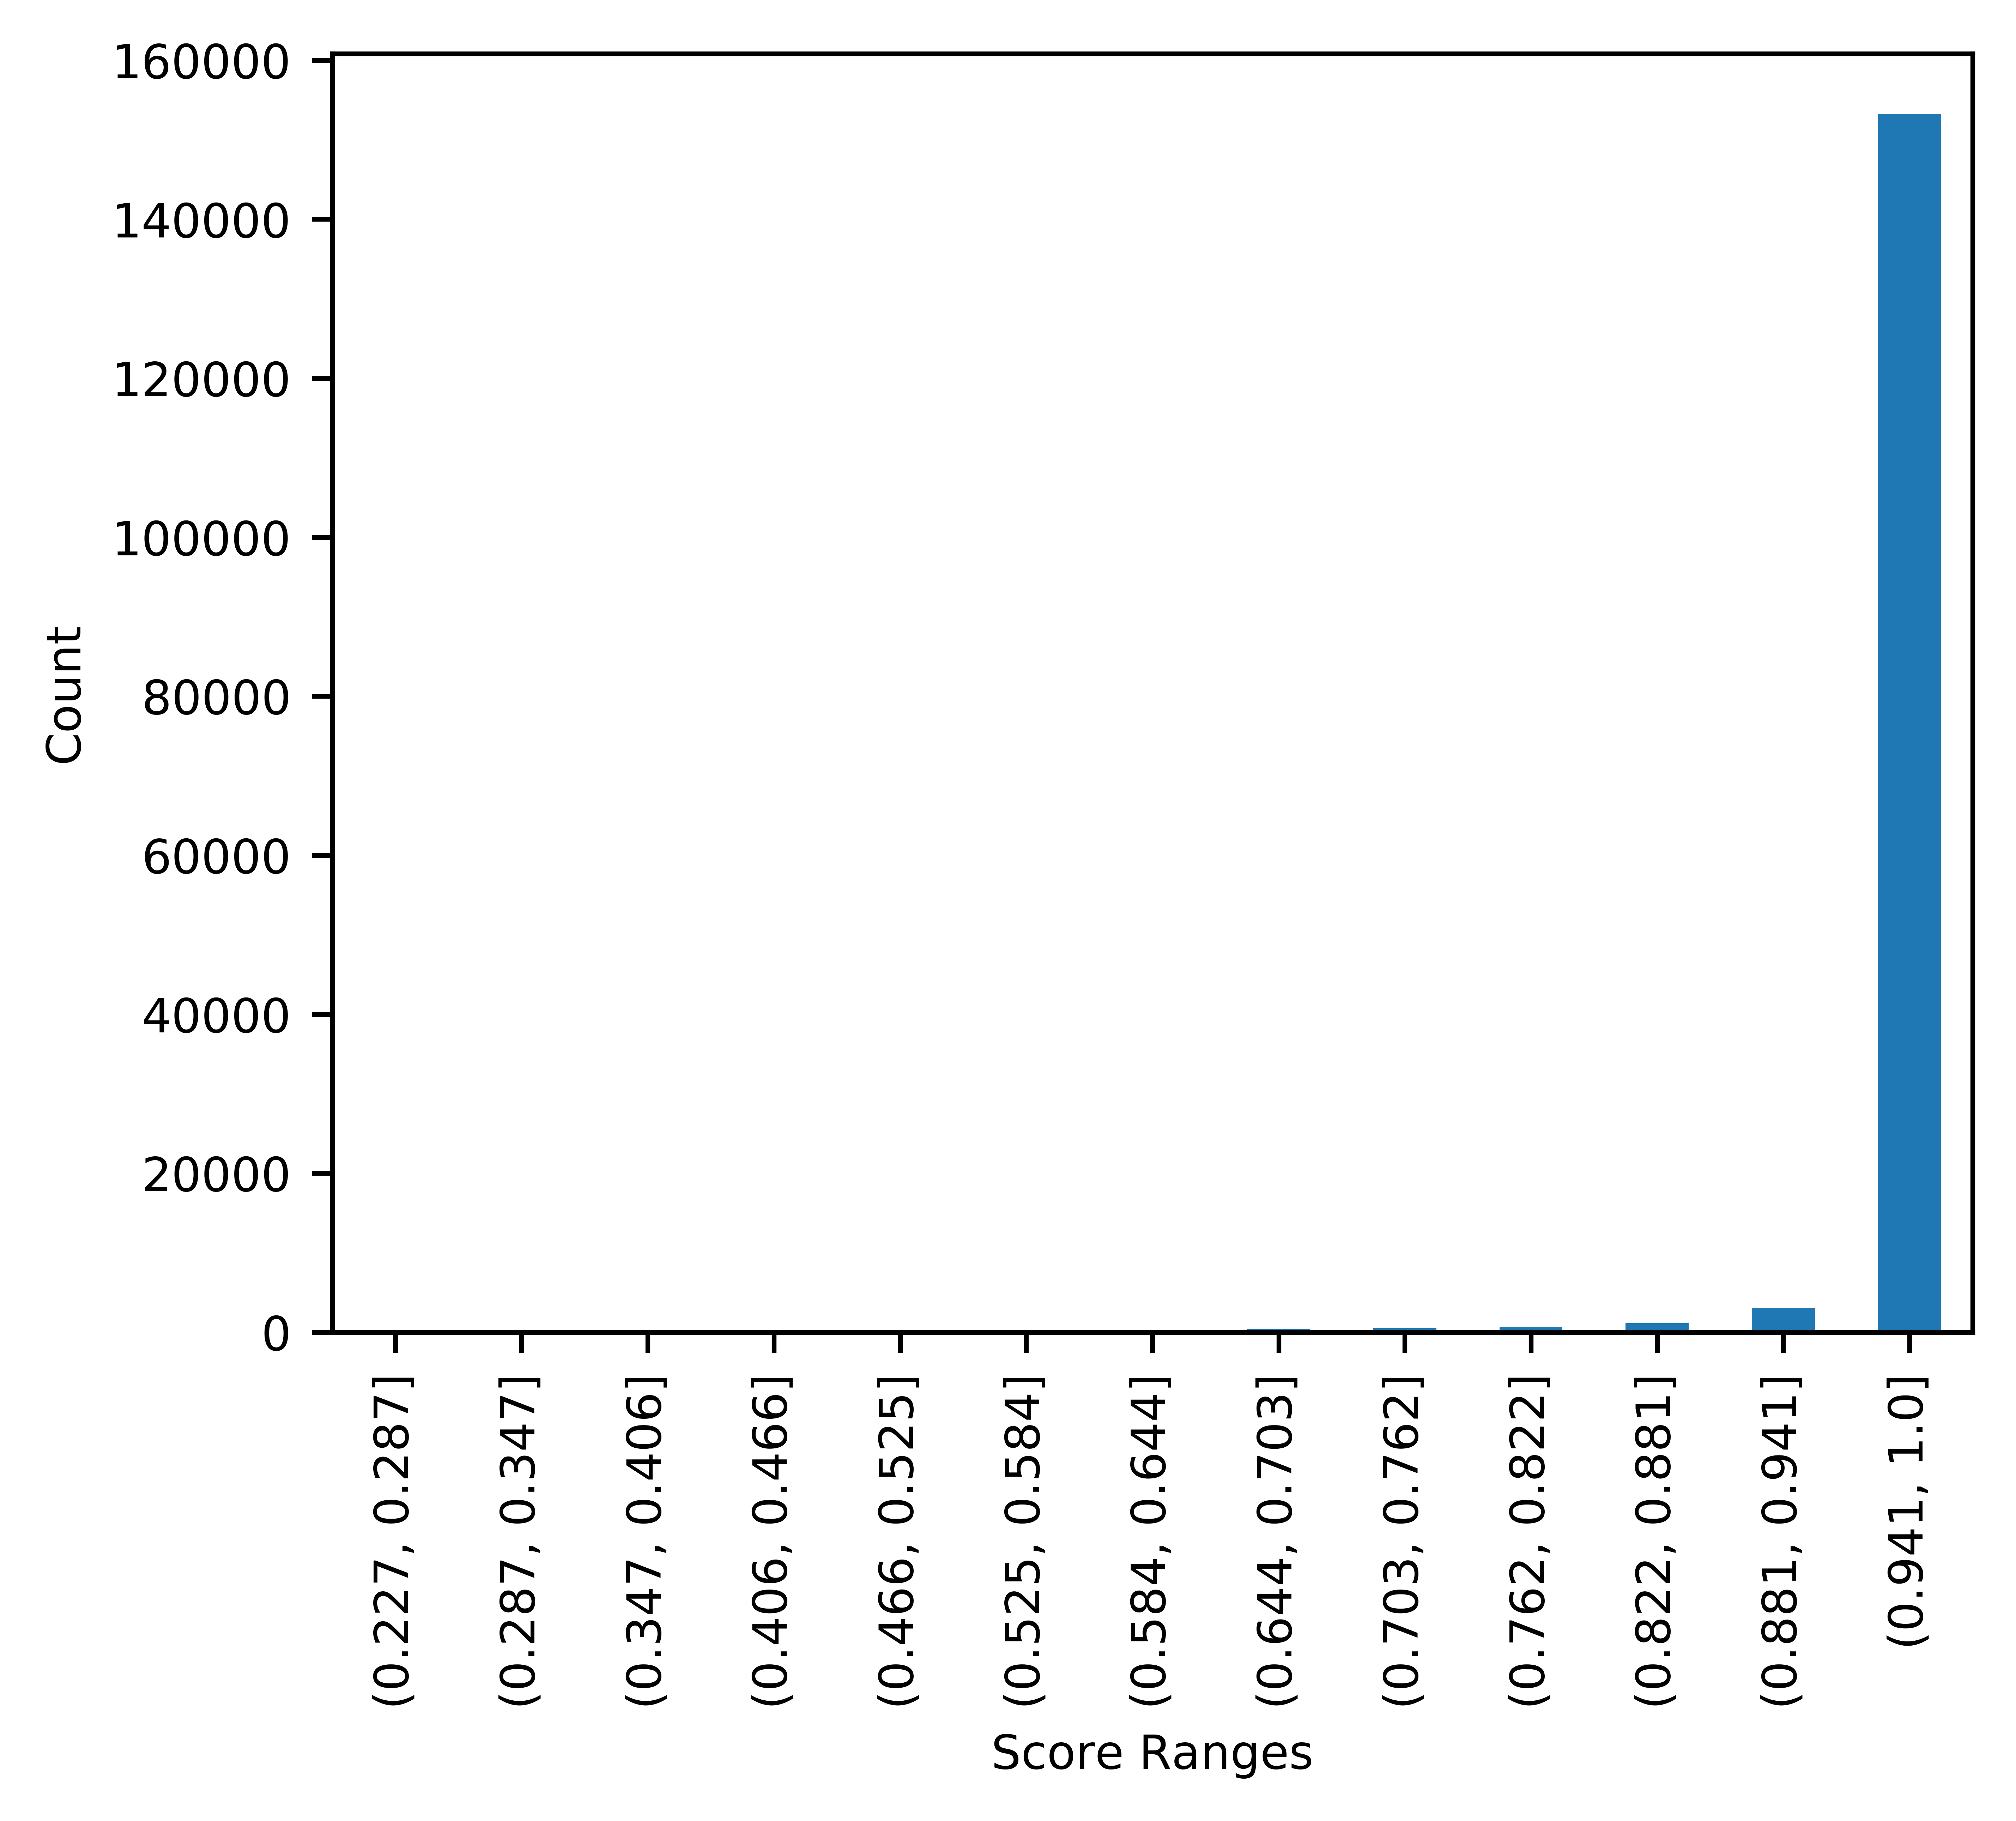
\includegraphics{./Figures/Ch_7_Results/IMG_Result_Distribution.png}
 \caption{Testing data score ranges distribution.}~\label{Fig:Results_Distribution}
\end{figure}


Another interesting example shows how the model can understand the pattern without \textit{tashkeel}, and the effect of adding \textit{tashkeel} to the text. We take the second row from Table~\ref{Tab:Results_Article}. In the case without \textit{tashkeel}, the model automatically tried to find any sequence of characters that follows any of the meter patterns. The model registered only the pattern including the \textit{tafa'il}, not the mean of the text. The model could therefore successfully detect a sequence of characters which follows \textit{Al-Taweel} with score 0.9988. In the case with \textit{tashkeel}, the model understood the new pattern of \textit{tafa'il} and gave the text low probability, below the threshold, and classified it as non-poem (not related to the 16 classic meters) with score 0.8390. This illustrates how \textit{tashkeel} can add a feature for model understanding to the \textit{tafa'il} pattern of the poem.

\textbf{Example:}

\begin{Arabic}
 \begin{traditionalpoem}
 يَعِدْ بُرْنُمُثْ بَوَّابَةَ صَلَاحِ لِلْعَوْدَةْ\quad & \quad لِتَّسْجِيلِ هَذَا المَوْسِمِ فِي بِرِمِرْلِجْ \\

 {\color{purple} يَعِدْبُرْ} {\color{blue} نُمُثْبَوَّا} {\color{OliveGreen} بَةَصَلَا} {\color{Brown} حِلِلْعَوْدَةْ}\quad & \quad
 {\color{purple} لِتَّسْجِي } {\color{blue} لِهَذَاالْمَوْ} {\color{OliveGreen} سِمِفِى } {\color{Brown} بِرِمِرْلِجْ}\\

 {\color{purple} \texttt{0/0//}} {\color{blue} \texttt{0/0/0//}} {\color{OliveGreen} \texttt{//{\color{red} /}0/}} {\color{Brown} \texttt{0/0/0//}}\quad & \quad {\color{purple} \texttt{/{\color{red} 0/0}0/}} {\color{blue} \texttt{0/0/0//}} {\color{OliveGreen} \texttt{//{\color{red} /0/}}} {\color{Brown} \texttt{//{\color{red} 0/}0/}}\\
 
 {\color{purple} \texttt{0/0//}} {\color{blue} \texttt{0/0/0// }} {\color{OliveGreen} \texttt{0/0//}} {\color{Brown} \texttt{0/0///}}\quad & \quad
 {\color{purple} \texttt{0/0//}} {\color{blue} \texttt{0/0/0//}} {\color{OliveGreen} \texttt{0/0//}} {\color{Brown} \texttt{0//0//}}\\
  
 {\color{purple} فَعُوْلُنْ} {\color{blue} مَفَاعِيْلُنْ} {\color{OliveGreen} فَعُولُن} {\color{Brown} مَفَاعِلُنْ}\quad & \quad
 {\color{purple} فَعُوْلُنْ} {\color{blue} مَفَاعِيْلُنْ} {\color{OliveGreen} فَعُوْلُنْ} {\color{Brown} مَفَاعِيْلُنْ}

 \end{traditionalpoem}
\end{Arabic}




\clearpage

\section{Discussion}\label{Sec:Discussion}

In this section, we discuss some points regarding our experiments and results, highlighting aspects we think it need more discussion or exploration.


\subsection{Dataset Unbalanced}

Our dataset was unbalanced, which certainly affected the results. Some significant drops are apparent in per-class accuracy, most of which concern the data size issue. We contend further work is required regarding this point, to reconstruct the experiments with balanced data, for example, 10k samples per class, and the results should be checked. Another approach could be to increase the size of the small classes to be at least 5\% of the overall classes’ percentage; this would enhance the learning accuracy of these classes. 

\subsection{Encoding Method}

Although in theory all the encoding methods which carry the same information should produce the same results, in practice, Deep Neural Networks showed this is not the case. To explain the reason, consider how Neural Network works with different encoding mechanism.

The encoding method is a transformer function $\mathcal{T}$. This function transforms a discrete input values $X$. We can denote to the values as a transformed feature $\mathcal{T}(X)$, the output of this transformer method. The output $\mathcal{T}(X)$ of this transformer in the new encoding space will be input to the Neural Network model. The model should be able to ``decode'' this type of encoding. Since the lossless encoding is inevitable, it is clear that for any two functions and any two encodings $\eta_1\left(\mathcal{T}_1(X)\right) = \left(\eta_1\cdot\mathcal{T}_1\cdot \mathcal{T}_2^{-1} \right)\left(\mathcal{T}_2(X)\right)$. This means that if the network $\eta_1$ is the most accurate network which can ``decode'' the encoding function (transformer) $\mathcal{T}_1$, this network $\eta_1$ is not a general network which can understand any encoding function. Moreover, to design this network requires a very complex architecture. Hence, if we have another encoding function $\mathcal{T}_2$ and we attempt to use the same network for the $\mathcal{T}_2$, designing another network is required $\eta_2 = \eta_1\cdot\mathcal{T}_1\cdot \mathcal{T}_2^{-1}$. However, this network may be need complicated architecture to ``decode'' the complicated pattern of $\mathcal{T}_2(X)$.


In general, any encoding function $\mathcal{T}$ requires a special network $\eta$ to obtain the correct decoding (learning) for the dataset. Our comparison between the encoding methods in the same Neural Networks architecture is therefore not accurate, as each requires different network design. However, all will reach the same results but over a different time; or there can be a small difference due to the inaccurate network architecture. Moreover, our work illustrates clearly the effects of the encoding methods; and comparing them, we believe the \textit{two-hot} encoding is the more suitable method to work with character level problems. It is the middle approach between \textit{one-hot}, which needs a huge amount of memory, and \textit{binary} which loses some meaning with the Arabic language diacritics effect.


\subsection{Weighting Loss Function}
Our weighting loss function does not solve the small classes issues (although the best model accuracy is achieved with weighting loss, but this is not a consistent result). The weighting loss function needs to be redesigned to solve this issue with the combination of learning rate and the batch size.

\subsection{Neural Network Configurations}

During our work, we show the effect of different network configurations on the model learning and accuracy. We conducted a range of experiments to find the best development architecture to facilitate make our experiments. In the beginning, the experiments took around 1.5 hours. Secondly, we proposed the multi-batch training to utilize parallel processing and prepare the data to the model faster, as our data was voluminous. We used enhanced an LSTM cell which reduced our experiments’ duration to 7-9 minutes per epoch, based on the architecture of the network.


We also showed the effect of network layers on learning and accuracy results. Hence, conducting more experiments with more deep layers and more complex architecture can facilitate the acquisition of more language knowledge and build a more complex model which will enhance both the per-class accuracy and the overall accuracy.

\subsection{Model Assessment}
In our work, we proposed the overall accuracy score as the model assessment method for the results. However, we need to highlight that the overall model accuracy produced from the Deep Neural Networks was very close to the overall accuracy score calculated from the confusion matrix, and in some experiments was almost the same. We also explored various statistical ways, for example $F_1$ score, to assess our model and we find the model results will be the same.


%%% Local Variables:
%%% mode: latex
%%% TeX-master: "../master"
%%% TeX-engine: xetex
%%% End:
